\documentclass[11pt,a4paper,openright]{report}
\usepackage[utf8]{inputenc}
\usepackage[T1]{fontenc}
\usepackage[bookmarks,
            breaklinks,
            hidelinks,
            backref=false,
            pdfhighlight=/I,
            pdffitwindow=true,
            pdfstartview=Fit,
            pdfcenterwindow=true,
            linkbordercolor={1 1 1},
            linkcolor=violetMy,
            urlcolor=violetMy,
            pdftitle=Calculation~of~predictions~for~non-identical~particle~correlations~in~AA~collisions~at~LHC~energies~from~hydrodynamics-inspired~models,
            pdfauthor=Mateusz~Galazyn]%
           {hyperref}
\usepackage{tabularx}
\usepackage{multirow}
\usepackage{amsmath,amssymb,xfrac}
\usepackage{tikz}
\usepackage{natbib}
\usepackage{datetime}
\usepackage{color,graphicx}
\usepackage{listings}
\usepackage{placeins}
\usepackage{url}
\usepackage{indentfirst}
\usepackage{lineno}
\usepackage{morefloats}
\usepackage{times}
\usepackage{pdfpages}
\usepackage{palatino}
\usepackage[polish,british]{babel}
\graphicspath{{figures/}}
\renewcommand\floatpagefraction{.9}
\renewcommand\topfraction{.9}
\renewcommand\bottomfraction{.9}
\renewcommand\textfraction{.1}
%\renewcommand\marginpar@font{\color{grey}}

\setlength{\emergencystretch}{8em}

\addtolength{\textwidth}{1cm}
\addtolength{\hoffset}{-0.5cm}

\title{Calculation of predictions for non-identical particle correlations in AA collisions at LHC energies from hydrodynamics-inspired models}
\author{Mateusz Gałażyn \\  \centering Warsaw University of Technology, Faculty of Physics}
\date{September 2014}

\begin{document}
\selectlanguage{british}
\newdateformat{mydatePL}{\THEDAY.0\THEMONTH.\THEYEAR~r.}
\newdateformat{mydateEN}{\monthname[\THEMONTH] \THEDAY, \THEYEAR}
\hyphenation{therminator}

\definecolor{violetMy}{rgb}{1,1,1}

\newcommand{\HRule}{\rule{\linewidth}{0.1mm}} % Defines a new command for the horizontal lines, change thickness here

\begin{titlepage}
	
\includegraphics[height=3.5cm]{wut}
	    \hfill
	
\includegraphics[height=3.5cm]{wut_physics}

	\center
	{\textbf{}}\\[3.3cm]
	{ \Huge Calculation of predictions for non-identical particle correlations in AA collisions at LHC energies from hydrodynamics-inspired models}
	\\[3cm]

	\LARGE\uppercase{Master of Science Thesis}\\[1.3cm]
		\begin{flushright} \Large
		Author:\hspace{2.cm}~\\
		\textbf{Mateusz Wojciech Gałażyn}\\[-0.5cm]
		\end{flushright}

		\begin{flushright} \Large
		Supervisor:\hspace{1.6cm}~\\
		\textbf{Prof.~Adam~{Kisiel}}\hspace{1.1cm}~\\[0.0cm]
		\end{flushright}

	{\large Warsaw,~\mydateEN\today}
	\vfill
\end{titlepage}	
\cleardoublepage

\begin{titlepage}
\selectlanguage{polish}
	
\includegraphics[height=3.5cm]{wut}
	    \hfill
	
\includegraphics[height=3.5cm]{wut_physics}
	\center
	{\textbf{}}\\[2cm]
	{ \Huge Obliczenia teoretycznych przewidywań korelacji cząstek nieidentycznych w zderzeniach AA przy energiach LHC pochodzących z modeli hydrodynamicznych }
	\\[3.2cm]


	\LARGE\uppercase{Praca magisterska}\\[1.3cm]
		\begin{flushright} \Large
		Autor:\hspace{2.2cm}~\\
		\textbf{Mateusz Wojciech Gałażyn}\\[-0.5cm]
		\end{flushright}

		\begin{flushright} \Large
		Promotor:\hspace{1.8cm}~\\
		\textbf{dr~hab.~inż.~Adam~{Kisiel}, prof. PW}\\[0cm]
		\end{flushright}

	{\large Warszawa,~\mydatePL\today}
	\vfill
\end{titlepage}
\cleardoublepage
\selectlanguage{british}
\linenumbers

\begin{abstract}
% !TEX root = ../main.tex
% An english abstract

This thesis presents results of two-particle momentum correlations analysis for different kinds of particles produced in heavy ion collisions.
The studies were carried for the data from lead-lead collisions at the centre of mass energy $\sqrt{s_{NN}}~=~2.76$~TeV simulated in the \verb|THERMINATOR| model using the (3+1)-dimensional hydrodynamic model with viscosity.
Analysis was performed for the three particle kinds: pions, kaons and protons for the collisions in eight different centrality ranges.

The \verb|THERMINATOR| model allows to perform statistical hadronization of stable particles and unstable resonances from a given hypersurface which is followed by the resonance propagation and decay phase.
The four-dimensional hypersurface is coming from the calculations performed on a basis of relativistic hydrodynamic framework with the viscosity corrections.

One can investigate space-time characteristics of the particle-emitting source through two-particle interferometry using experimental observables.
The experimental-like analysis of the data coming from a model calculations yields a possibility to test the hydrodynamic description of a quark-gluon plasma.
This thesis concentrates on the verification of the prediction of appearance of femtoscopic radii scaling with the transverse mass.

The three dimensional correlation functions were calculated using spherical harmonics decomposition.
One can use this approach to perform calculations with lower statistics and moreover the visualization of results is much easier.
The calculated correlation functions show expected increase of a correlation for pions and kaons at the low relative momenta of a pair.
For the protons at the same momentum region, the decrease occurs.
The transverse pair momentum and centrality dependence on a correlation function is observed.
In order to perform the quantitative analysis of this influence, the fitting of theoretical formula for correlation function was performed.
The femtoscopic radii calculated in the LCMS and PRF are falling with the transverse mass $m_T$.
To test the scaling predicted from the hydrodynamics, the power law was fitted $\alpha m_T^{-\beta}$.
The radii calculated for pions, kaons and protons in the LCMS are following the common scaling.
In case of the PRF no such scaling is observed.
To recover the scaling in the PRF, the approximate factor is proposed: $\sqrt{ \left. \left( \sqrt{\gamma_T} + 2 \right) \middle/ 3 \right. }$.
The radii in the PRF divided by the proposed scaling factor are falling on the common curve, therefore the scaling can be recovered using the proposed scaling factor.
The experimental analysis is usually performed in the PRF (requires less statistics), hence the method of scaling recovery enables easier testing of the hydrodynamic predictions, which are not visible in the PRF.

\end{abstract}
\cleardoublepage
\renewcommand{\abstractname}{Streszczenie}
\begin{abstract}
\selectlanguage{polish}
\hyphenation{po-prze-czną}
% a polish abstract
\end{abstract}
\selectlanguage{british}
\cleardoublepage
\pagestyle{empty}
\pagenumbering{gobble}
\tableofcontents
\cleardoublepage
\pagestyle{headings}
\pagenumbering{arabic}

% !TEX root = ../main.tex
\chapter*{Introduction}
\addcontentsline{toc}{chapter}{Introduction}
Many people were trying to discover what was in the beginning of the Universe which we observe today.
Through the years, more or less successful theories were appearing and trying to describe its origin and behaviour.
Among them is one model, which provides a comprehensive explanation for a broad range of phenomena, including the cosmic microwave background, abundance of the light elements and Hubble's law.
This model is called The Big Bang theory and has born in 1927 on the basis of principles proposed by the Belgian priest and scientist Georges Lema{\^i}tre.
Using this model and known laws of physics one can calculate the characteristics of the Universe in detail back in time to the extreme densities and temperatures.
However, at some point these calculations fail.
The extrapolation of the expansion of the Universe backwards in time using general relativity yields an infinite density and temperature at a finite time in the past.
This appearance of singularity is a signal of the breakdown of general relativity.
The range of this extrapolation towards singularity is debated - certainly we can go no closer than the end of \textit{Planck epoch} i.e. $10^{-43}$~s.
At this very first era the temperature of the Universe was so high, that the four fundamental forces - electromagnetism, gravitation, weak nuclear interaction and strong nuclear interaction - were one fundamental force.
Between $10^{-43}$~s and $10^{-36}$~s of a lifetime of the Universe, there is a \textit{grand unification epoch}, at which forces are starting to separate from each other.
The \textit{electroweak epoch} lasted from $10^{-36}$~s to $10^{-12}$~s, when the strong force separated from the electroweak force.
After the electroweak epoch, there was the \textit{quark epoch} in which the Universe was a dense ``soup'' of quarks.
During this stage the fundamental forces of gravitation, electromagnetism, strong and weak interactions had taken their present forms. 
The temperature at this moment was still too high to allow quarks to bind together and form hadrons.
At the end of quark era, there was a big freeze-out - when the average energy of particle interactions had fallen below the binding energy of hadrons.
This era, in which quarks became confined into hadrons, is known as the \textit{hadron epoch}.
At this moment the matter had started forming nuclei and atoms, which we observe today.

Here arises the question: how can we study the very beginning of the Universe?
To do this, one should create in a laboratory a system with such a large density and high temperature to recreate those conditions.
Today, this is achievable through sophisticated machines, which are particle accelerators.
In the particle accelerators, like the Large Hadron Collider at CERN, Geneva or Relativistic Heavy Ion Collider at Brookhaven National Laboratory in Upton, New York, the heavy ions after being accelerated to near the speed of light are collided in order to generate extremely dense and hot phase of matter and recreate the quark-gluon plasma.
The plasma is believed to behave like an almost ideal fluid and to become a medium, that can be described by the laws of relativistic hydrodynamics.

This thesis is providing predictions for collective behaviour of the quark-gluon plasma coming from the hydrodynamic equations.
Experimental-like analysis was performed for the high energy Pb-Pb collisions generated with \verb|THERMINATOR| model.

The 1st chapter is an introduction to the theory of heavy ion collisions.
It contains the brief description of the Standard Model and Quantum Chromodynamics.
The quark-gluon plasma and its signatures are also characterized.

In the 2nd chapter, the relativistic hydrodynamic framework and the \verb|THERMINATOR| model used to perform the simulations of collisions are characterized.

The 3rd chapter covers the particle interferometry method used in this work.
The effects coming from the hydrodynamics in the experimental results for particle interferometry are also presented.
An algorithm of building experimental correlation functions is also described in this chapter.

In the 4th chapter, a detailed analysis of the results for two-particle femtoscopy for different pairs of particles is presented.
The quantitative analysis of calculated femtoscopic radii as well as the appearance of transverse mass scaling is discussed.
\newpage
% !TEX root = ../main.tex
\chapter{Theory of heavy ion collisions}
  %
  % ========
  \section{The Standard Model}
  % ========
    In the 1970s, a new theory of fundamental particles and their interaction emerged.
    It was a new concept, which combines the electromagnetic, weak and strong nuclear interactions between know particles.
    This theory is called \textit{The Standard Model}.
    There are seventeen named particles in the standard model, organized into the chart shown below (Fig. \ref{fig:standard_model}).
    Fundamental particles are divided into two families: \textit{fermions} and \textit{bosons}.
     \begin{figure}[h]
       \centering
       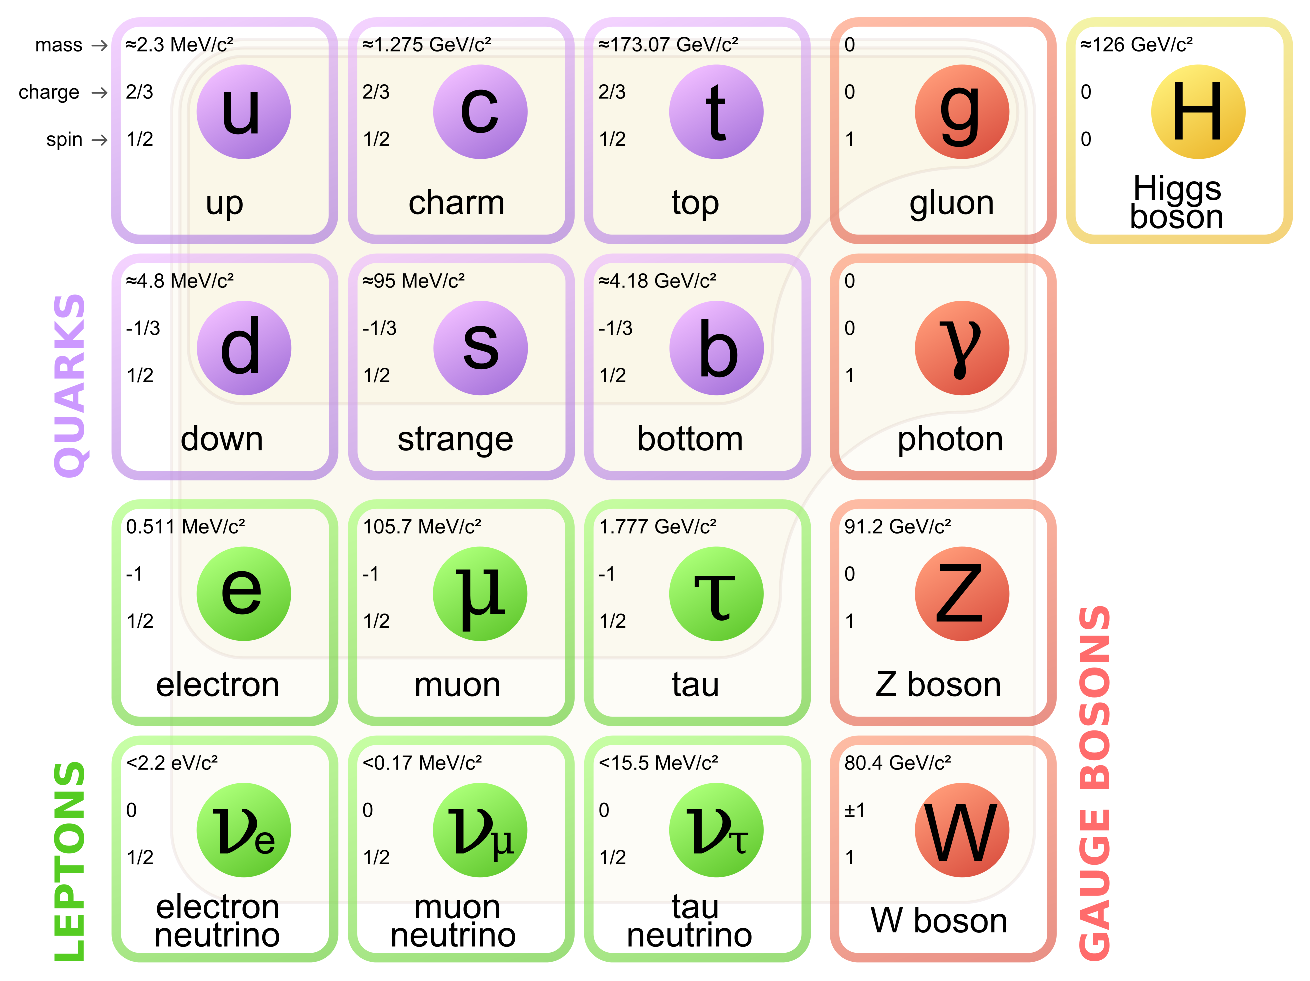
\includegraphics[width=0.9\textwidth]{standard_model}
       \caption{The Standard Model of elementary particles~\cite{sm_svg}.}
       \label{fig:standard_model}
     \end{figure}
     
    Fermions are the building blocks of matter.
    They are divided into two groups.
    Six of them, which must bind together are called \textit{quarks}.
    Quarks are known to bind into doublets (\textit{mesons}), triplets (\textit{baryons}) and recently confirmed four-quark states.\footnote{The LHCb experiment at CERN in Geneva confirmed recently the existence of $Z$(4430) - a particle consisting of four quarks~\cite{fourquark}.}
    Two of baryons, with the longest lifetimes, are forming a nucleus: a proton and a neutron.
    A proton is build from two up quarks and one down, and neutron consists of two down quarks and one up.
    A proton is found to be a stable particle (at least it has a lifetime larger than $10^{35}$ years) and a free neutron has a mean lifetime about $8.8\times10^2$ s.
    Fermions, that can exist independently are called \textit{leptons}.
    Neutrinos are a subgroup of leptons, which are only influenced by weak interaction.
    Fermions can be divided into three generations (three columns in the Figure \ref{fig:standard_model}).
    Generation I particles can combine into hadrons with the longest life spans. 
    Generation II and III consists of unstable particles which also form unstable hadrons. 
    
    Bosons are force carriers.
    There are four fundamental forces: weak - responsible for radioactive decay, strong - coupling quarks into hadrons, electromagnetic - between charged particles and gravity - the weakest, which causes the attraction between particles with mass.
    The Standard Model describes the first three.
    The weak force is mediated by $W^{\pm}$ and $Z^0$ bosons, electromagnetic force is carried by photons $\gamma$ and the carriers of a strong interaction are gluons \textit{g}.
    The fifth boson is a Higgs boson which is responsible for giving other particles mass. 
 
  %
  % ========
  \section{Quantum Chromodynamics}
  % ========
    %
    % ========
    \subsection{Quarks and gluons}
    % ========
      Quarks interact with each other through the strong interaction.
      The mediator of this force is a \textit{gluon} - a massless and electrical chargeless particle.
      In the quantum chromodynamics (QCD) - theory describing strong interaction - there are six types of ``charges'' (like electrical charges in the electrodynamics) called \textit{colours}.
      The colours were introduced because some of the observed particles, like $\Delta^{-}$, $\Delta^{++}$ and $\Omega^{-}$ appeared to consist of three quarks with the same flavour (\textit{ddd}, \textit{uuu} and \textit{sss} respectively), which was in conflict with the Pauli principle.
      One quark can carry one of the three colours (usually called \textit{red}, \textit{green} and \textit{blue}) and antiquark one of the three anti-colours respectively.
      Only colour-neutral (or white) particles could exist.
      Mesons are assumed to be a colour-anticolour pair, while baryons are \textit{red-green-blue} triplets.
      Gluons also are colour-charged and there are 8 types of gluons.
      Therefore they can interact with themselves~\cite{perkins}.
    %
    % ========
    \subsection{Quantum Chromodynamics potential}
    % ========
      As a result of the fact that gluons are massless, one can expect, that the static potential in QCD will have the form like similar one in electrodynamics e.g. \mbox{$\sim 1/r$} (through analogy to photons).
      In reality the QCD potential is assumed to have the form of~\cite{perkins}
      \begin{equation}
        V_s = - \frac{4}{3} \frac{\alpha_s}{r} + kr~,
        \label{eq:qcd_potential}
      \end{equation}
      where the $\alpha_s$ is a coupling constant of the strong force and the $kr$ part is related with \textit{confinement}.
      In comparison to the electromagnetic force, a value of the strong coupling constant is $\alpha_s \approx 1$ and the electromagnetic one is $\alpha = 1/137$.

      The fact that quarks does not exist separately and are always bound, is called confinement.
      As two quarks are pulled apart, the linear part $kr$ in the Eq.~\ref{eq:qcd_potential} becomes dominant and the potential becomes proportional to the distance.
      This situation resembles stretching of a string.
      At some point, when the string is so large it is energetically favourable to create a quark-antiquark pair.
      At this moment such pair (or pairs) is formed, the string breaks and the confinement is preserved (Fig. \ref{fig:string_break}).
      \begin{figure}[h]
        \centering
        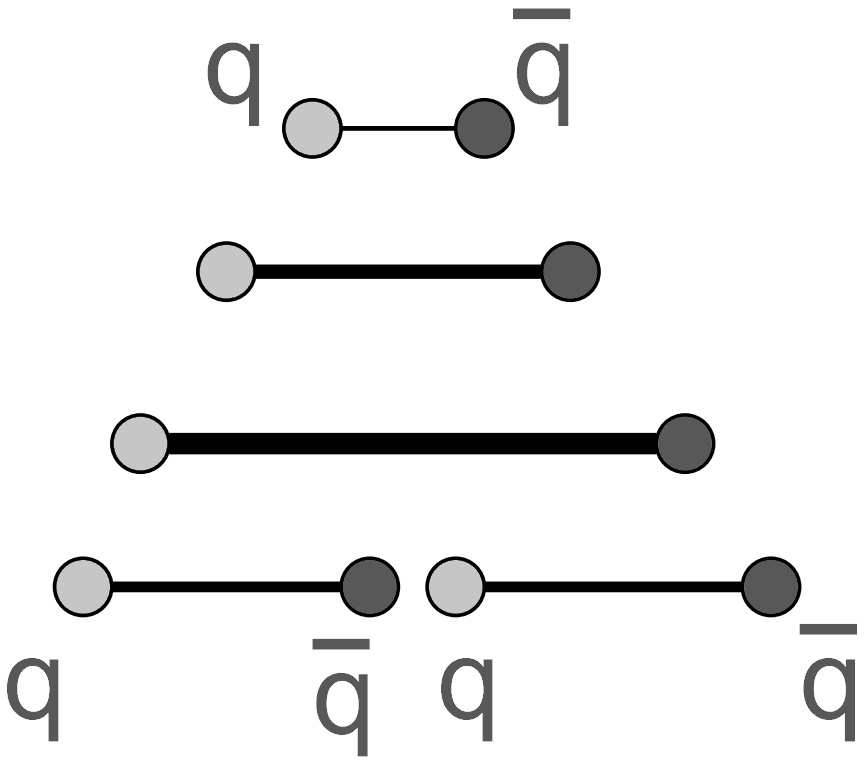
\includegraphics[width=0.25\textwidth]{string_break}
        \caption{A string breaking and a creation of a new quark-anti-quark pair~\cite{dfck}.}
        \label{fig:string_break}
      \end{figure}
      
      On the other hand, for small $r$, an interaction between the quarks and gluons is dominated by the Coulomb-like term $-\frac{4}{3} \frac{\alpha_s}{r}$.
      The coupling constant $\alpha_s$ depends on the four-momentum $Q^2$ transferred in the interaction.
      This dependence is presented in Fig.~\ref{fig:strong_cc}.
      \begin{figure}[h]
        \centering
        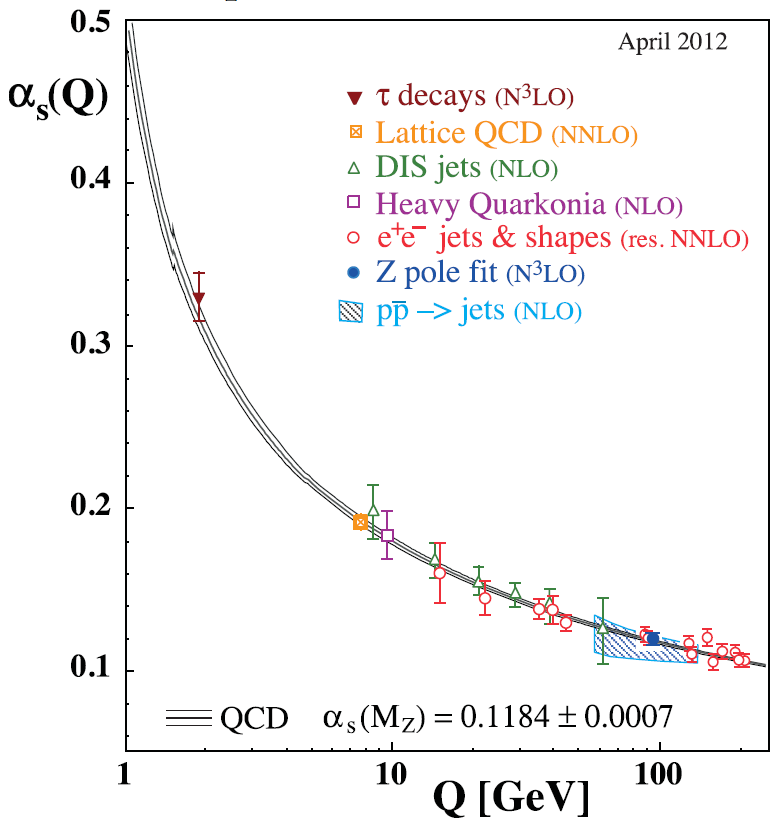
\includegraphics[width=0.55\textwidth]{strong_cc}
        \caption{The coupling parameter $\alpha_s$ dependence on four-momentum transfer~$Q^2$~\cite{pdg}.}
        \label{fig:strong_cc}
      \end{figure}
      \begin{figure}[h]
        \centering
        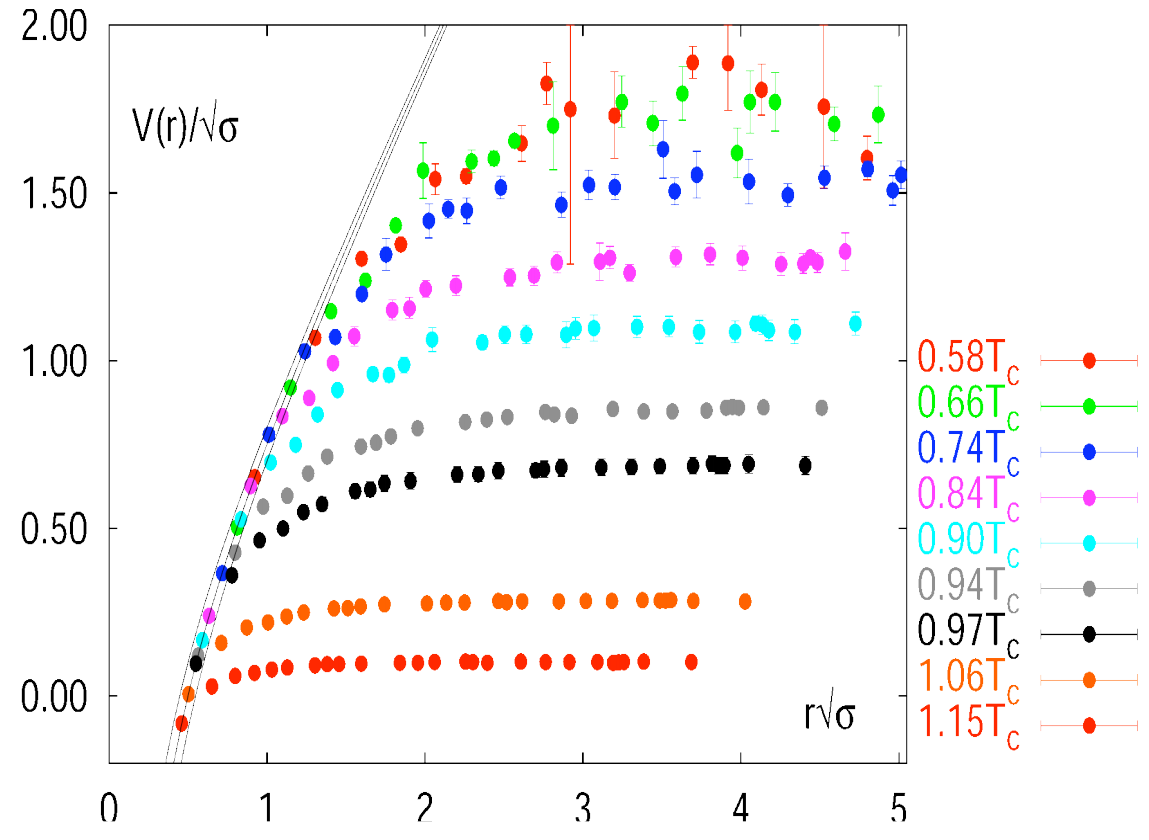
\includegraphics[width=0.65\textwidth]{qcd_potential_t}
        \caption{The QCD potential for a quark-antiquark pair as a function of distance for different temperatures. A value of a potential decreases with the temperature~\cite{dfck}.}
        \label{fig:qcd_potential}
      \end{figure}
      The value $\alpha_s$ decreases with increasing momentum transfer and the interaction becomes weak for large $Q^2$, i.e. $\alpha_s (Q) \to 0$.
      Because of the weakening of coupling constant, quarks at large energies (or small distances) are starting to behave like free particles.
      This phenomenon is known as \textit{asymptotic freedom}.      
      The QCD potential also has temperature dependence - the force strength ``melts'' with the temperature increase.
      Therefore the asymptotic freedom is expected to appear in either the case of high baryon densities (small distances between quarks) or very high temperatures.
      This temperature dependence is illustrated in Fig.~\ref{fig:qcd_potential}.
      
      If the coupling constant $\alpha_s$ is small, one can use perturbative methods to calculate physical observables.
      Perturbative QCD (pQCD) successfully describes hard processes (with large $Q^2$), such as jet production in high energy proton-antiproton collisions.
      The applicability of pQCD is defined by the \textit{scale parameter} $\Lambda_{QCD} \approx$~200~MeV.
      If $Q \gg \Lambda_{QCD}$ then the process is in the perturbative domain and can be described by pQCD.
      A description of soft processes (when $Q <$~1~GeV) is a problem in QCD - perturbative theory breaks down at this scale.
      Therefore, to describe processes with low $Q^2$, one has to use alternative methods like Lattice QCD.
      Lattice QCD (LQCD) is non-perturbative implementation of a field theory in which QCD quantities are calculated on a discrete space-time grid.
      LQCD allows to obtain properties of matter in equilibrium, but there are some limitations.
      Lattice QCD requires fine lattice spacing to obtain precise results - therefore large computational resources are necessary.
      With the constant growth of computing power this problem will become less important.
      The second problem is that lattice simulations are possible only for baryon density $\mu_B = $~0.
      At $\mu_B \neq 0$, Lattice QCD breaks down because of the sign problem.
      In QCD the thermodynamic observables are related to the grand canonical partition function, which has a baryonic chemical potential $\mu_B$ as a parameter.
      Therefore, the baryonic density can be controlled by tuning the baryonic chemical potential.
      For fermions $\mu_B$ can be both positive and negative.
      For a particles with $\mu_B$, their antiparticles have chemical potentials with opposite sign $-\mu_B$.
      Since at the early universe the number of baryons and antibaryons were almost equal we can use $\mu_B=0$ to a very good approximation~\cite{qcd_fodor}.
    %
    % ========
    \subsection{The quark-gluon plasma}
    % ========
      The new state of matter in which quarks are no longer confined is known as a \textit{quark-gluon plasma} (QGP).
      The predictions coming from the discrete space-time Lattice QCD calculations reveal a phase transition from the hadronic matter to the quark-gluon plasma at the high temperatures and baryon densities.
      \begin{figure}[b]
        \centering
        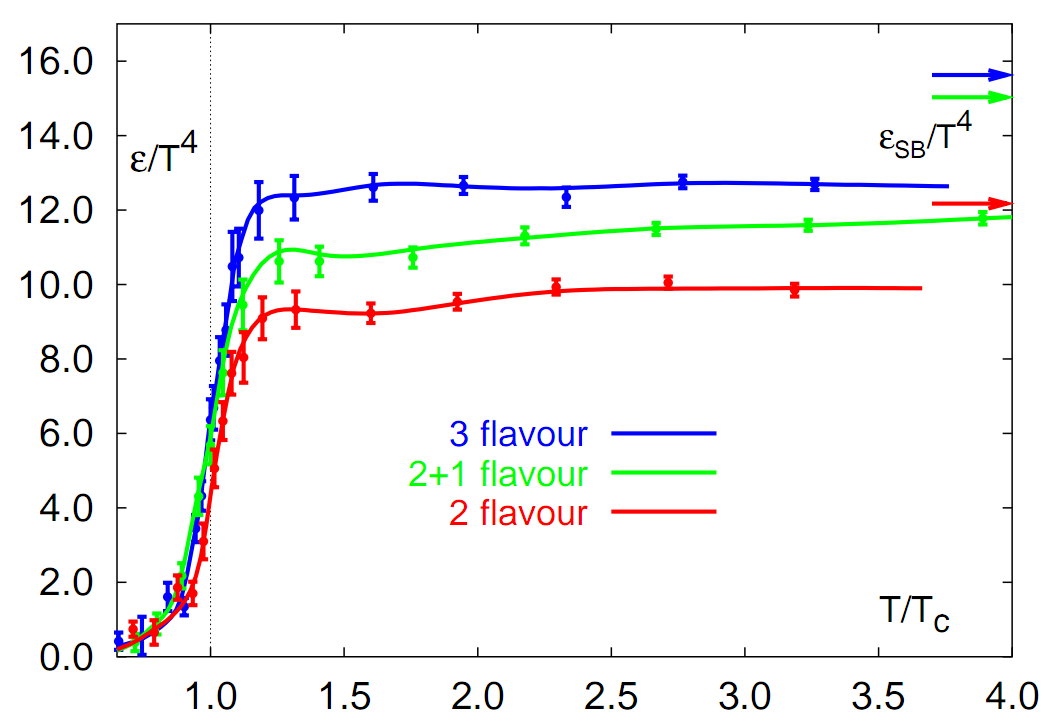
\includegraphics[width=0.68\textwidth]{lqcd}
        \caption{A number of degrees of freedom as a function of a temperature~\cite{karsch}.}
        \label{fig:lqcd}
      \end{figure}
      The results obtained from such calculations are shown on Fig.~\ref{fig:lqcd}.
      The energy density $\epsilon$ which is divided by $T^4$ is a measure of the number of degrees of freedom in the system.
      One can observe significant rise of this value, when the temperature increases past the critical value $T_C$.
      Such increase is signaling a phase transition - the formation of QGP~\cite{drkisiel}.
      The values of the energy densities plotted in Fig.~\ref{fig:lqcd} do not reach the Stefan-Boltzmann limit $\epsilon_{SB}$ (marked with arrows), which corresponds to an ideal gas.
      This can indicate some residual interactions in the system.
      According to the results from the RHIC\footnote{Relativistic Heavy Ion Collider at Brookhaven National Laboratory in Upton, New York}, the new phase of matter behaves more like an ideal fluid, than like a gas~\cite{bartke}.
      \begin{figure}[t]
        \centering
        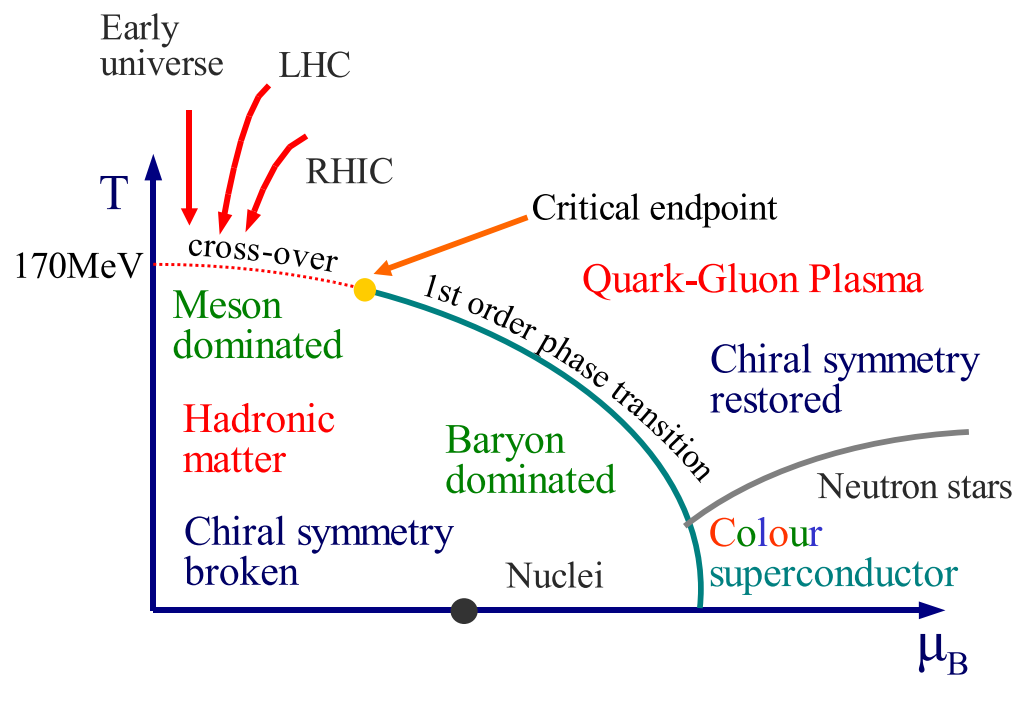
\includegraphics[width=0.7\textwidth]{phase_diagram}
        \caption{Phase diagram coming from the Lattice QCD calculations~\cite{drkisiel}.}
        \label{fig:phase_diagram}
      \end{figure}

      One of the key questions, to which current heavy ion physics tries to find an answer is the value of a critical temperature $T_C$ as a function of a baryon chemical potential $\mu_B$ (baryon density), where the phase transition occurs.
      The results coming from the Lattice QCD are presented in Fig.~\ref{fig:phase_diagram}.
      The phase of matter in which quarks and gluons are deconfined is expected to exist at large temperatures.
      In the region of small temperatures and high baryon densities, a different state is supposed to appear - a \textit{colour superconductor}.
      The phase transition between hadronic matter and the QGP is thought to be of 1$^\text{st}$ order at $\mu_B \gg 0$.
      However as $\mu_B \to 0$ quarks' masses become significant and a sharp transition transforms into a rapid but smooth cross-over.
      It is believed that in Pb-Pb collisions observed at the LHC\footnote{Large Hadron Collider at CERN, Geneva}, the created matter has high enough temperature to be in the quark-gluon plasma phase, then cools down and converts into hadrons, undergoing a smooth transition~\cite{drkisiel}.
  %
  % ========
  \section{Relativistic heavy ion collisions}
  % ========
    %
    % ========
    \subsection{Stages of heavy ion collision}
    % ========

      To create the quark-gluon plasma one has to achieve high enough temperatures and baryon densities.
      Such conditions can be recreated in the heavy ion collisions at the high energies.
      \begin{figure}[h]
        \centering
        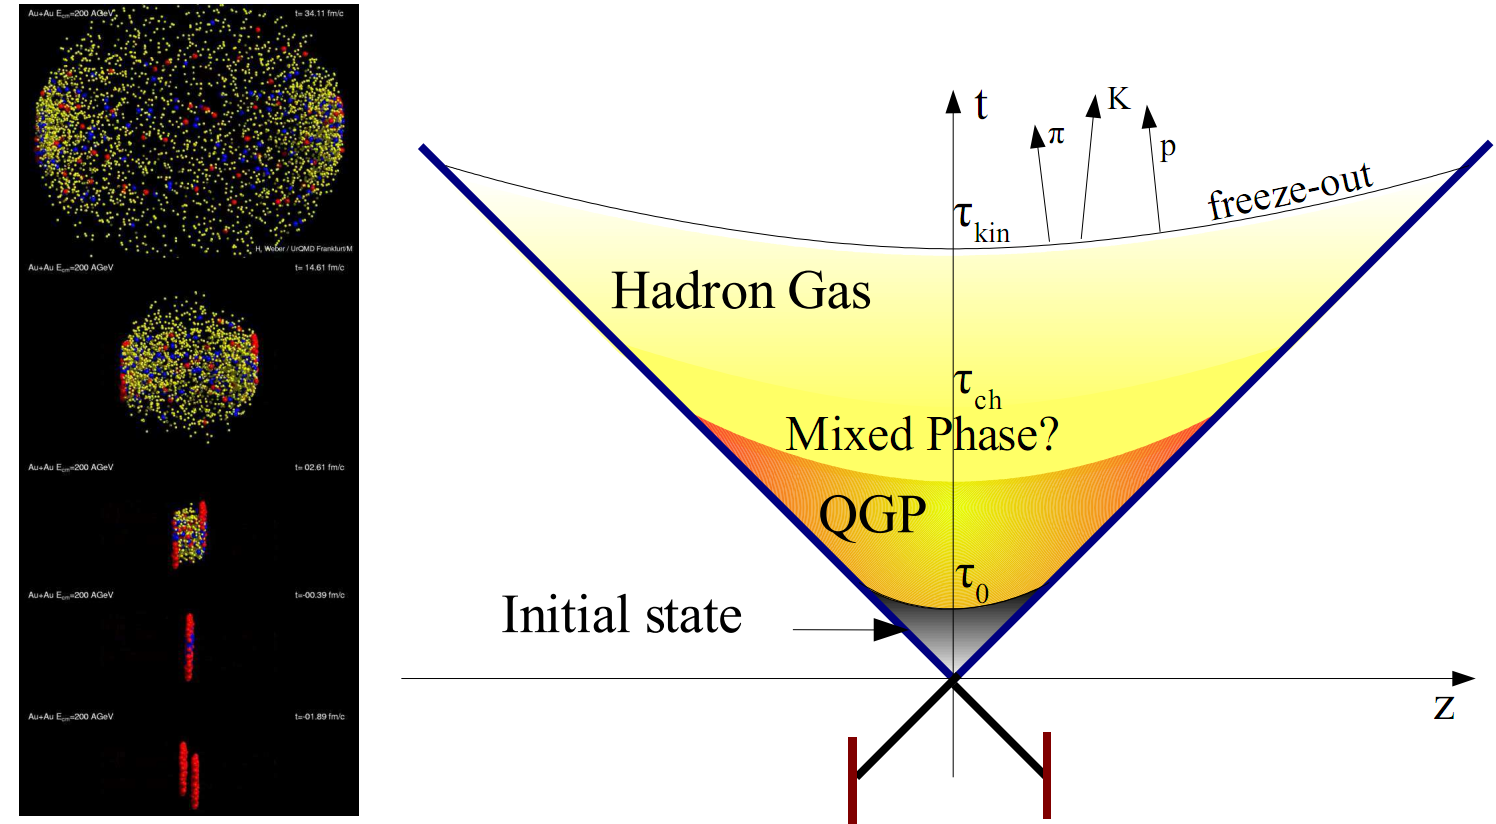
\includegraphics[width=1\textwidth]{collision}
        \caption{Left: stages of a heavy ion collision simulated in the UrQMD model. Right: schematic view of a heavy ion collision evolution~\cite{drkisiel}.}
        \label{fig:colision}
      \end{figure}
      The left side of the Figure~\ref{fig:colision} shows simplified picture of a central collision of two highly relativistic nuclei in the centre-of-mass reference frame.
      The colliding nuclei are presented as thin disks because of the Lorentz contraction.
      In the central region, where the energy density is the highest, a new state of matter - the quark-gluon plasma - is supposedly created.
      Afterwards, the plasma expands ad cools down, quarks combine into hadrons and their mutual interactions cease when the system reaches the \textit{freeze-out} temperature.
      Subsequently, produced free hadrons move towards the detectors.

      On the right side of the Figure~\ref{fig:colision} a space-time evolution of a collision process is presented, plotted in the light-cone variables (z, t).
      The two highly relativistic nuclei are traveling basically along the light cone until they collide at the centre of the diagram. 
      Nuclear fragments emerge from the collision again along the (forward) light cone, while the matter between fragmentation zones populates the central region.
      This hot and dense matter is believed to be in the state of the quark-gluon plasma.
      Several frameworks exist to describe this transition to the QGP phase, for example: QCD string breaking, QCD parton cascades or colour glass condensate evolving into glasma and later into quark-gluon plasma~\cite{florkowski}.
      \paragraph{String breaking}
      In the string picture, the nuclei pass through each other forming colour strings.
      This is analogous to the situation depicted in the Fig~\ref{fig:string_break} -  the colour string is created between quarks inside particular nucleons in nuclei.
      In the next step strings decay~/~fragment forming quarks and gluons or directly hadrons.
      This approach becomes invalid at very high energies, when the strings overlap and cannot be treated as independent objects.
      \paragraph{Parton cascade}
      The parton\footnote{A parton is a common name for a quark and a gluon.} cascade model is based on the pQCD.
      The colliding nuclei are treated as clouds of quarks which penetrate through each other.
      The key element of this method is the time evolution of the parton phase-space distributions, which is governed by a relativistic Boltzmann equation with a collision term that contains dominant perturbative QCD interations.
      The bottleneck of the parton cascade model is the low energies regime, where the $Q^2$ is too small to be described by the perturbative theory.
      \paragraph{Colour glass condensate}
      The colour glass condensate assumes, that the hadron can be viewed as a tightly packed system of interacting gluons.
      The saturation of gluons increases with energy, hence the total number of gluons may increase without bound.
      Such a saturated and weakly coupled gluon system is called a colour glass condensate.
      The fast gluons in the condensate are Lorentz contracted and redistributed on the two very thin sheets representing two colliding nuclei.
      The sheets are perpendicular to the beam axis.
      The fast gluons produce mutually orthogonal colour magnetic and electric fields, that only exist on the sheets.
      Immediately after the collision, i.e. just after the passage of the two gluonic sheets through each other, the longitudinal electric and magnetic fields are produced forming the \textit{glasma}.
      The glasma fields decay through the classical rearrangement of the fields into radiation of gluons.
      Also decays due to the quantum pair creations are possible.
      In this way, the quark-gluon plasma is produced.


      Interactions within the created quark-gluon plasma bring the system into the local statistical equilibrium, hence its further evolution can be described by the relativistic hydrodynamics.
      The hydrodynamic expansion causes the system to become more and more dilute.
      The phase transition from the quark-gluon plasma to the hadronic gas occurs.
      Further expansion causes a transition from the strongly interaction hadronic gas to weakly interacting system of hadrons which move freely to the detectors.
      Such decoupling of hadrons is called the \textit{freeze-out}.
      The freeze-out can be divided into two phases: the chemical freeze-out and the thermal one.
      The \textit{chemical freeze-out} occurs when the inelastic collisions between constituents of the hadron gas stop.
      As the system evolves from the chemical freeze-out to the thermal freeze-out the dominant processes are elastic collisions (such as, for example $\pi+\pi\to$ $\rho \to$ $\pi+\pi$) and strong decays of heavier resonances which populate the yield of stable hadrons.
      The \textit{thermal freeze-out} is the stage of the evolution of matter, when the strongly coupled system transforms to a weakly coupled one (consisting of essentially free particles).
      In other words this is the moment, where the hadrons practically stop to interact.
      Obviously, the temperatures corresponding to the two freeze-outs satisfy the condition
      \begin{equation}
        T_{chem} > T_{therm}~,
      \end{equation}
      where $T_{chem}$ (inferred from the ratios of hadron multiplicities) is the temperature of the chemical freeze-out, and $T_{therm}$ (obtained from the investigation of the transverse-momentum spectra) is the temperature of the thermal freeze-out~\cite{florkowski}.

    %taken from grebieszkow's HIP 7th lecture - HIC dynamics
    %
    % ========
    \subsection{QGP signatures}
    % ========
      The quark-gluon plasma is a very short living and unstable state of matter.
      One cannot investigate the properties of a plasma and confirm its existence directly.
      Hence, the several experimental effects were proposed as QGP signatures, some of them have been already observed in heavy ion experiments~\cite{drkisiel}.
      As matter created in the heavy ions collisions is supposed to behave like a fluid, one should expect appearance of collective behaviour at small transverse momenta - so called \textit{elliptic flow} and \textit{radial flow}.
      The next signal is the temperature range obtained from the measurements of \textit{direct photons}, which gives us information, that the system created in heavy ion collisions is far above the critical temperature obtained from the LQCD calculations.
      The \textit{puzzle in the di-lepton spectrum} can be explained by the modification of spectral shape of vector mesons (mostly $\rho$ meson) in the presence of a dense medium.
      This presence of a medium can also shed light on the \textit{jet quenching} phenomenon - the suppression occurence in the high $p_T$ domain.
      \subsubsection{Elliptic flow}
        \begin{figure}[b]
          \centering
          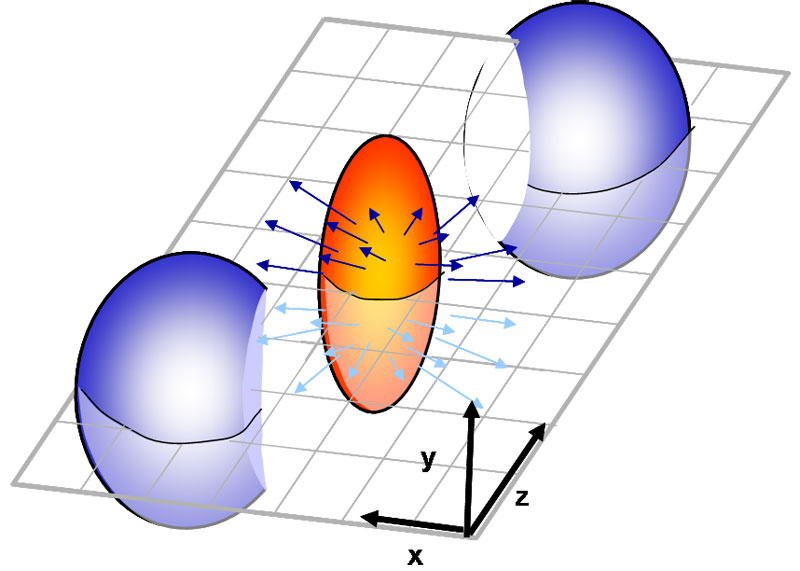
\includegraphics[width=0.5\textwidth]{elliptic_flow}
          \caption{Overlapping region which is created in heavy ion collisions has an almond shape. Visible x-z plane is a \textit{reaction plane}. The x-y plane is a \textit{transverse plane}. The z is a direction of the beam~\cite{eflow}.}
          \label{fig:elliptic_flow}
        \end{figure}
        In a non-central heavy ion collisions, created region of matter has an almond shape with its shorter axis in the \textit{reaction plane} (Fig.~\ref{fig:elliptic_flow}).
        The pressure gradient is much larger in-plane rather than out-of-plane.
        This causes larger acceleration and transverse velocities in-plane rather than out-of-plane.
        Such differences can be investigated by studying the distribution of particles with respect to the reaction plane orientation~\cite{hip}:
        \begin{equation}
          E\frac{d^3 N}{d p^3} = \frac{1}{2\pi} \frac{d^2 N}{p_T d p_T d y} (1 + 2 v_1 \cos(\phi) + 2 v_2 \cos(2 \phi) + ...)~,
          \label{eq:elliptic_flow}
        \end{equation}
        where $\phi$ is the angle between particle transverse momentum $p_T$ (a momentum projection on a transverse plane) and the reaction plane, $N$ is a number of particles and $E$ is an energy of a particle.
        The $y$ variable is \textit{rapidity} defined as:
        \begin{equation}
          y = \frac{1}{2} \ln \left( \frac{E+ p_L}{E - p_L} \right)~,
        \end{equation}
        where $p_L$ is a longitudinal component of a momentum (paralel to the beam direction).
        The $v_n$ coefficients indicate the shape of a system.
        For the most central collisions (b = 0 - see Fig.~\ref{fig:impact_parameter}) all coefficients vanish $\bigwedge_{n \in N_{+}} v_n = 0$ (the overlapping region has the spherical shape).
        \begin{figure}[b]
          \centering
          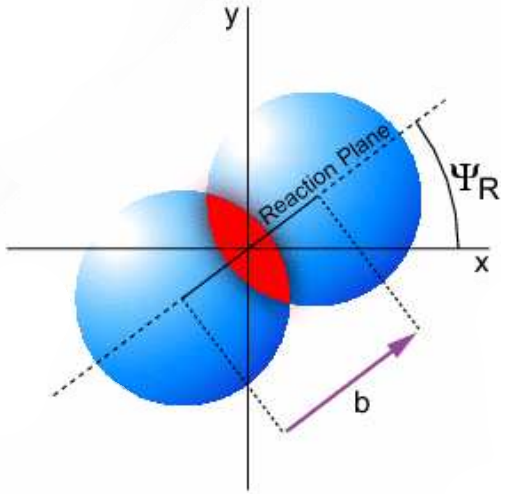
\includegraphics[width=0.4\textwidth]{impact}
          \caption{Cross-section of a heavy ion collision in a transverse plane. 
          %$\Psi_R$ is an angle between transverse plane and the reaction plane. 
          The \textit{b} parameter is an \textit{impact parameter} - a distance between centers of nuclei during a collision. An impact parameter is related with the centrality of a collision and a volume of the quark-gluon plasma~\cite{hip}.}
          \label{fig:impact_parameter}
        \end{figure}
        The Fourier series elements in the parentheses in Eq.~\ref{eq:elliptic_flow} represent different kinds of flow.
        The first value: ``1'' represents the \textit{radial flow} - an isotropic flow in every direction.
        Next coefficient $v_1$ is responsible for \textit{direct flow}.
        The $v_2$ coefficient is a measure of elliptic anisotropy (\textit{elliptic flow}).
        The $v_2$ has to build up in the early stage of a collision - later the system becomes too dilute: space asymmetry and the pressure gradient vanish.
        Therefore the observation of elliptic flow means that the created matter was in fact a strongly interacting matter.
        \begin{figure}[h]
          \centering
          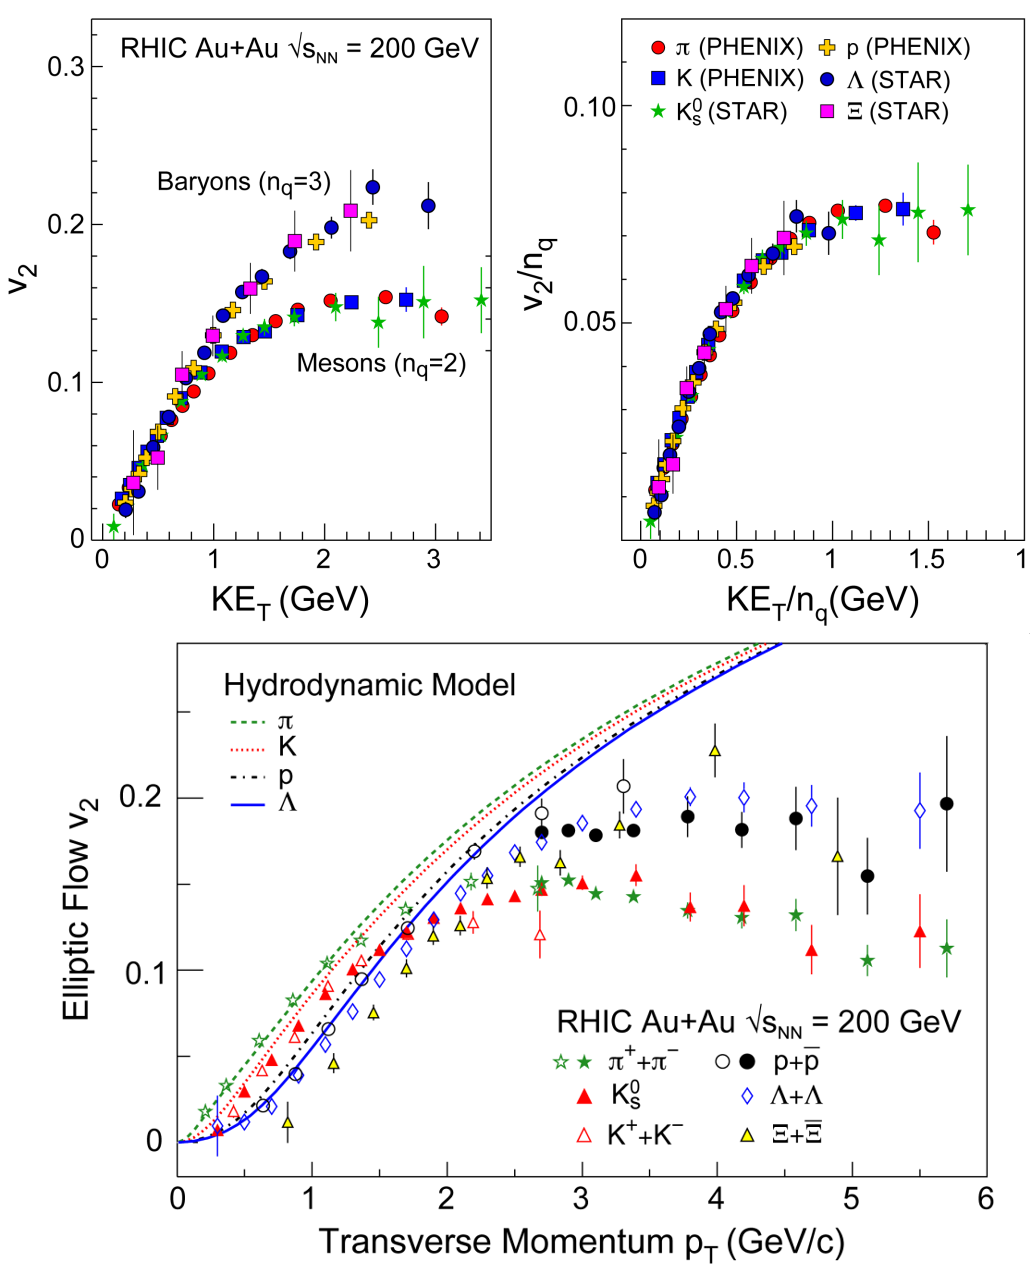
\includegraphics[width=0.82\textwidth]{elliptic_flow_experimental}
          \caption{\textit{Lower:} The elliptic flow $v_2$ follows the hydrodynamical predictions for an ideal fluid perfectly. Note that $> 99\%$ of all final hadrons have $p_T < 1.5$~GeV/c. \textit{Upper left:} The $v_2$ plotted versus transverse kinetic energy $KE_T = m_T - m_0 = \sqrt{p_T^2 + m_0^2} - m_0$. The $v_2$ follows different universal curves for mesons and baryons. \textit{Upper right:} When scaled by the number of valence quarks, the $v_2$ follows the same universal curve for all hadrons and for all values of scaled transverse kinetic energy~\cite{heinz}.}
          \label{fig:elliptic_flow_experimental}
        \end{figure}

        The $v_2$ coefficient was measured already at CERN SPS, LHC and RHIC.
        For the first time hydrodynamics successfully described the collision dynamics as the measured $v_2$ reached hydrodynamic limit (Fig.~\ref{fig:elliptic_flow_experimental}).
        As expected, there is a mass ordering of $v_2$ as a function of $p_T$ (lower plot in the Fig.~\ref{fig:elliptic_flow_experimental}) with pions having the largest and protons the smallest anisotropy.
        In the upper plots in the Fig.~\ref{fig:elliptic_flow_experimental} there is a $v_2$ as a function of transverse kinetic energy.
        The left plot shows two universal trend lines for baryons and mesons.
        After the scaling of $v_2$ and the kinetic energy by the number of valence quarks, all of the hadrons follow the same universal curve.
        Those plots show that strong collectivity is observed in heavy ion collisions.

      \FloatBarrier
      \subsubsection{Transverse radial flow}
        Elliptic flow described previously is caused by the pressure gradients which must also produce a more simple collective behaviour of matter - a~movement inside-out, called radial flow.
        Particles are pushed to higher momenta and they move away from the center of the collision.
        A source not showing collective behaviour, like pp collisions, produces particle spectra that can be fitted by a power-law~\cite{drkisiel}:
        \begin{equation}
          \frac{1}{2\pi p_T} \frac{d^2 N}{d p_T d \eta} = C \left( 1 +\frac{p_T}{p_0} \right)~.
        \end{equation}
        The $\eta$ variable is \textit{pseudorapidity} defined as follows:
        \begin{equation}
          \eta = \frac{1}{2} \ln \left( \frac{p + p_L}{p - p_L} \right) = -\ln \left(\frac{\theta}{2} \right)~,
        \end{equation}
        where $\theta$ is an emission angle $\cos \theta = p_L / p$~.
        \begin{figure}[h]
          \centering
          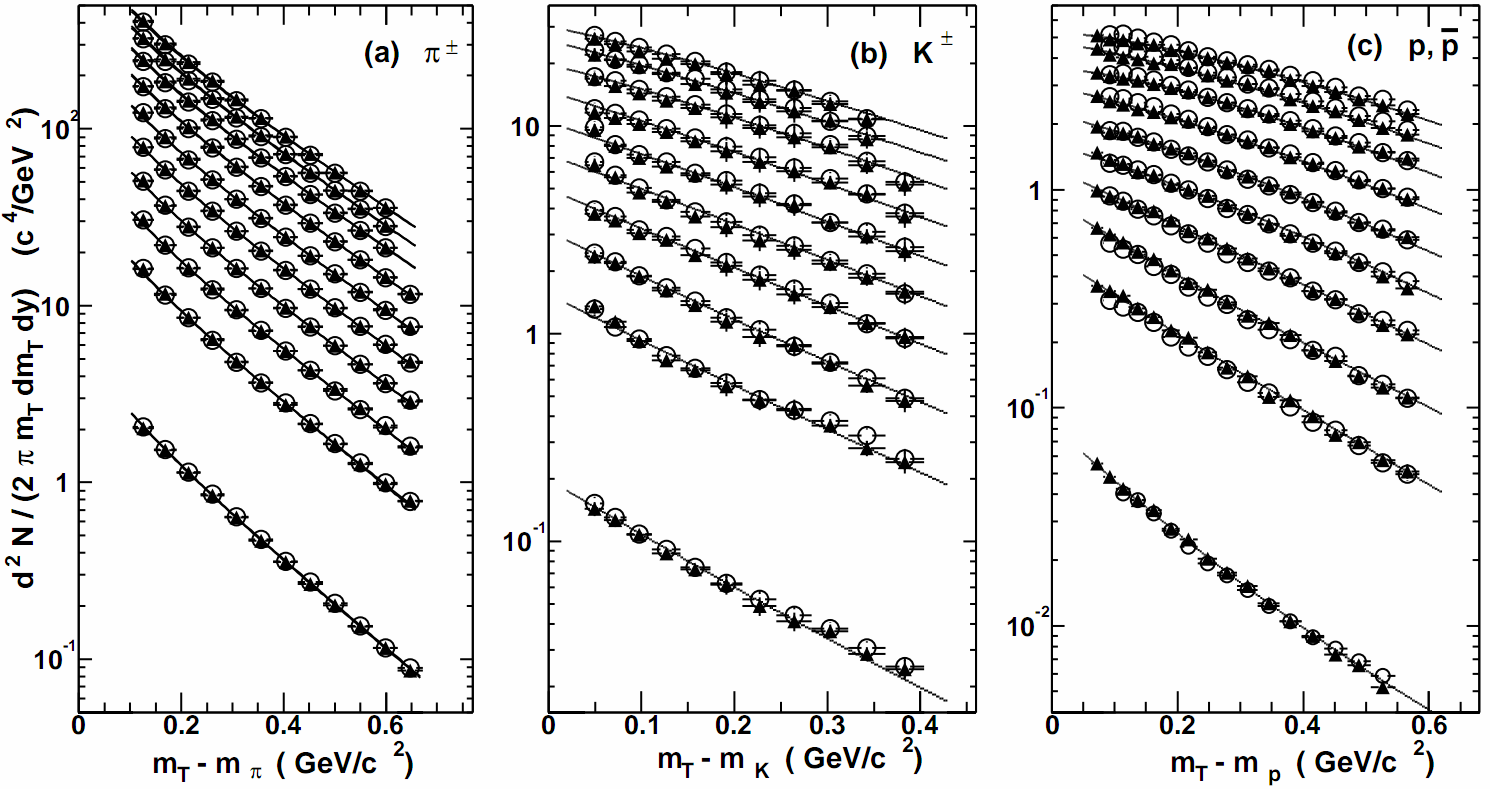
\includegraphics[width=1\textwidth]{mt_spectra}
          \caption{Invariant yield of particles versus transverse mass $m_T = \sqrt{p^2_T + m_0^2}$ for $\pi^{\pm}$, $K^{\pm}$, $p$ and $\bar{p}$ at mid-rapidity for p+p collisions (bottom) and Au+Au events from 70-80\% (second bottom) to 0-5\% (top) centrality~\cite{mtspectra}.}
          \label{fig:invariant_yield}
        \end{figure}

        The hydrodynamical expansion of a system gives the same flow velocity kick for different kinds of particles - ones with bigger masses will gain larger $p_T$ boost.
        This causes increase of the yield of particles with larger transverse momenta.
        In the invariant yield plots one can observe the decrease of the slope parameter, especially for the heavier hadrons.
        This is presented in the Fig.~\ref{fig:invariant_yield}.
        The most affected spectra are ones of kaons (b) and protons (c).
        One can notice decrease of the slope parameter for heavy ion collisions (plots from second bottom to top) comparing to the proton-proton collisions (bottom ones), where no boost from radial flow should occur~\cite{drkisiel}.

        Another signature of a transverse radial flow is a dependence of HBT radii on a pair transverse momentum.
        Detailed description of this effect is presented in the Section~\ref{ch:pi-scaling}.
      \subsubsection{Direct photons}
        The direct photons are photons, which are not coming from the final state hadrons decays.
        Their sources can be various interaction from charged particles created in the collision, either at the partonic or at the hadronic level.
        Direct photons are considered to be an excellent probe of the early stage of the collision.
        This is because their mean free path is very large when compared to the size of created system in the collision.
        Thus photons created at the early stage leave the system without suffering any interaction and retain information about this stage, in particular about its temperature.

        \begin{figure}[b]
          \centering
          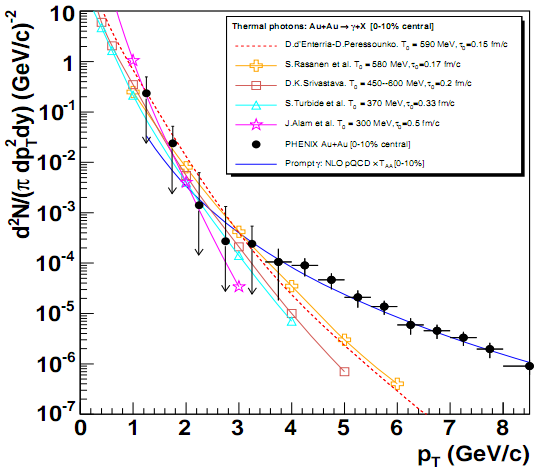
\includegraphics[width=0.7\textwidth]{direct_photons}
          \caption{Thermal photons spectra for the central Au+Au collisions at $\sqrt{s_{NN}}=$~200~GeV computed within different hydrodynamical models compared with the pQCD calculations (solid line) and experimental data from PHENIX (black dots)~\cite{rapp_xu}.}
          \label{fig:direct_photons}
        \end{figure}
        One can distinguish two kinds of direct photons: \textit{thermal} and \textit{prompt}.
        Thermal photons can be emitted from the strong processes in the quark-gluon plasma involving quarks and gluons or hot hadronic matter (e.g. processes: $\pi\pi \to \rho \gamma$, $\pi\rho \to \pi \gamma$).
        Thermal photons can be observed in the low $p_T$ region.
        Prompt photons are believed to come from ``hard'' collisions of initial state partons belonging to the colliding nuclei.
        The prompt photons can be described using the pQCD.
        They will dominate the high $p_T$ region.
        The analysis of transverse momentum of spectra of direct photons revealed, that the temperature of the source of thermal photons produced in heavy ion collisions at RHIC is in the range 300-600 MeV (Fig.~\ref{fig:direct_photons}).
        Hence the direct photons had to come from a system whose temperature is far above from the critical temperature for QGP creation.

      \subsubsection{Puzzle in di-lepton mass spectrum}
        The invariant mass spectra (Fig.~\ref{fig:di-lepton}) of lepton pairs reveal many peaks corresponding to direct decays of various mesons into a lepton pair.
        The continuous background in this plot is caused by the decays of hadrons into more than two leptons (including so-called \textit{Dalitz decays} into a lepton pair and a photon).
        \begin{figure}[h]
          \centering
          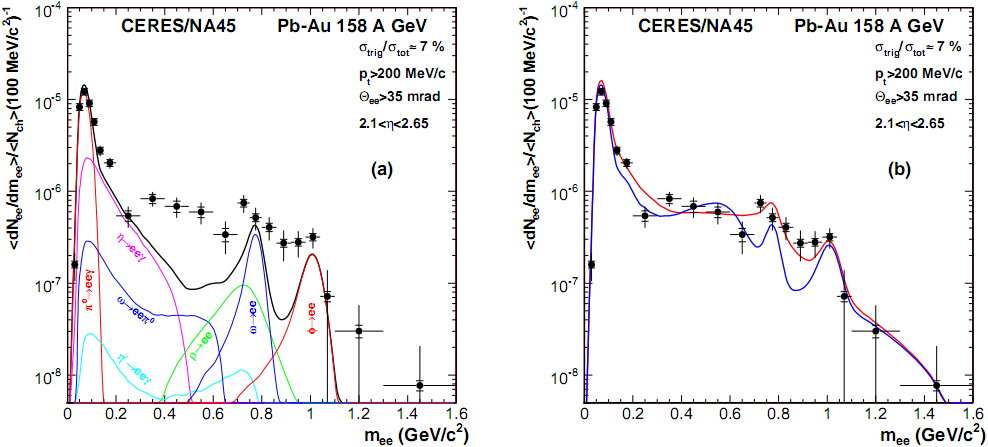
\includegraphics[width=1\textwidth]{di-lepton}
          \caption{Left: Invariant mass spectrum of $e^{+}$-$e^{-}$ pairs in Pb+Au collisions at 158\textit{A}~GeV compared to the sum coming from the hadron decays predictions. Right: The expectations coming from model calculations assuming a dropping of the $\rho$ mass (blue) or a spread of the $\rho$ width in the medium (red)~\cite{marin}.}
          \label{fig:di-lepton}
        \end{figure}
        Particular hadron decay channels, which contribute to this spectrum are shown in Fig.~\ref{fig:di-lepton} with the coloured lines and their sum with the black one.
        The sum (called \textit{the hadronic cocktail}) of various components describes experimental spectra coming from the simple collisions (like p+p or p+A) quite well with the statistical and systematical uncertainties~\cite{bartke}.
        This situation is different considering more complicated systems i.e. A+A.
        Spectra coming from Pb+Au collisions are presented on the plots in the Fig.~\ref{fig:di-lepton}.
        The ``hadronic cocktail'' does not describe the data, in the mass range between the $\pi$ and the $\rho$ mesons a significant excess of electron pairs over the calculated sum is observed.
        Theoretical explanation of this phenomenon assumes modification of the spectral shape of vector mesons in a dense medium.
        Two different interpretations of this increase were proposed: a decrease of meson mass with the medium density and increase of the meson width in the dense medium.
        In principle, one could think of simultaneous occurrence of both effects: mass shift and resonance broadening.
        Experimental results coming from the CERES disfavour the mass shift hypothesis indicating only broadening of resonance peaks (Fig.~\ref{fig:di-lepton}b)~\cite{bartke}.

      \subsubsection{Jet quenching}
        A jet is defined as a group of particles with close vector momenta and high energies.
        It has its beginning when the two partons are going in opposite directions and have energy big enough to produce new quark-antiquark pair and then radiate gluons.
        This process can be repeated many times and it results in two back-to-back jets of hadrons.
        It has been found that jets in the opposite hemisphere (\textit{away-side jets}) show a very different pattern in d+Au and Au+Au collisions.
        This is shown in the azimuthal correlations in the~Fig.~\ref{fig:di-jet}.
        In d+Au collisions, like in p+p, a pronounced away-side jet appears around $\Delta \phi = \pi$, exactly opposite to the trigger jet, which is typical for di-jet events.
        In central Au+Au collisions the away-side jet is suppressed. 
        \begin{figure}[b]
          \centering
          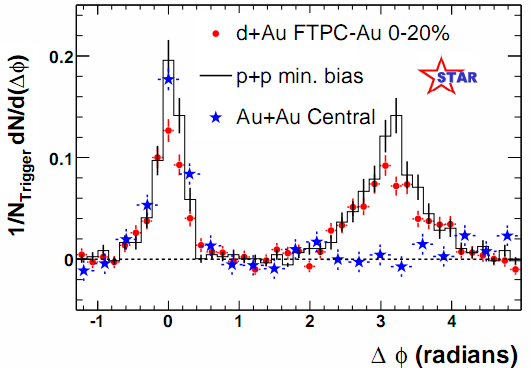
\includegraphics[width=0.7\textwidth]{dijet}
          \caption{Azimuthal angle difference $\Delta \phi$ distributions for different colliding systems at $\sqrt{s_{NN}}$ = 200 GeV. Transverse momentum cut: $p_T >$ 2 GeV. For the Au+Au collisions the away-side jet is missing~\cite{rhic_jets}.}
          \label{fig:di-jet}
        \end{figure}
        When the jet has its beginning near the surface of the quark-qluon plasma, one of the jets (\textit{near-side jet}) leaves the system almost without any interactions.
        This jet is visible on the correlation plot as a high peak at $\Delta \phi = 0$.
        However, the jet moving towards the opposite direction has to penetrate a dense medium.
        The interaction with the plasma causes energy dissipation of particles and is visible on an azimuthal correlation plot as a disappearance of the away-side jet~\cite{bartke}.


\newpage
% !TEX root = ../main.tex
\chapter{Therminator model}
  \verb|THERMINATOR|~\cite{therminator} is a Monte Carlo event generator designed to investigate the particle production in the relativistic heavy ion collisions.
  The functionality of the code includes a generation of the stable particles and unstable resonances at the chosen hypersurface model.
  It performs the statistical hadronization which is followed by space-time evolution of particles and the decay of resonances.
  The key element of this method is an inclusion of a complete list of hadronic resonances.
  The second version of \verb|THERMINATOR|~\cite{therminator2} comes with a posibility to incorporate any shape of freeze-out hypersurface and the expansion velocity field, especially those generated externally with various hydrodynamic codes.
  %
  % ========
  \section{Statistical hadronization}
  % ========
    Statistical description of heavy ion collision has been successfully used to describe quantitatively \textit{soft} physics, i.e. the regime with the transverse momentum not exceeding 2 GeV.
    The assumption that hadronic matter before rapid expansion reaches equilibrium, leads to good results in particle abundances measured in heavy ion experiments, in particular, at the high energies.
    At the rather high temperature of the freeze-out $\approx$140-160 MeV, the resonances contribute very significantly to the observables.
    Therefore, the crucial element for the success of the statistical approach is the complete inclusion of hadronic resonances~\cite{therminator}.
    %
    % ========
    \subsection{Cooper-Frye formalism}
    % ========
      % opisac wzor C-F

    %
    % ========
    \section{(3+1)-dimensional viscous hydrodynamics}
    % ========
    Most of the relativistic viscous hydrodynamic calculations are done in \mbox{(2+1)-dimensions}.
    Such simplification assumes boost-invariance of a matter created in a collision.
    Experimental data reveals that no boost-invariant region is formed in the collisions~\cite{chmeson}.
    Hence, for the better description of created system a \mbox{(3+1)-dimensional} model is required.

    In the four dimensional relativistic dynamics one can describe a system using a space-time four-vector $x^\nu=(ct,x,y,z)$, a velocity four-vector $u^\nu=\gamma(c,v_x,v_y,v_z)$ and a energy-momentum tensor $T^{\mu\nu}$.
    The particular components of $T^{\mu\nu}$ have a following meaning:
    \begin{itemize}
      \item $T^{00}$ - an energy density,
      \item $c T^{0\alpha}$ - an energy flux across a surface $x^\alpha$,
      \item $T^{\alpha0}$ - an $\alpha$-momentum flux across a surface  $x^\alpha$ multiplied by $c$,
      \item $T^{\alpha\beta}$ - components of momentum flux density tensor,
    \end{itemize}
    where $\gamma = (1-v^2/c^2)^{-1/2}$ is Lorentz factor and $\alpha,\beta \in \{1,2,3\}$.
    Using $u^\nu$ one can express $T^{\mu\nu}$ as follows~\cite{israel}:
    \begin{equation}
      \label{eq:visc_ten}
      T^{\mu\nu}_0 = (e+p)u^\mu u^\nu - pg^{\mu\nu}
    \end{equation}
    where $e$ is an energy density, $p$ is a pressure and $g^{\mu\nu}$ is an inverse metric tensor:
    \begin{equation}
      g^{\mu\nu} = 
      \begin{bmatrix}
        1 & 0 & 0 & 0 \\
        0 & -1 & 0 & 0 \\
        0 & 0 & -1 & 0 \\
        0 & 0 & 0 & -1
      \end{bmatrix} .
    \end{equation}
    The presented version of energy-momentum tensor (\ref{eq:visc_ten}) can be used to describe dynamics of a perfect fluid.
    To take into account influence of viscosity, one has to apply the following corrections coming from shear $\pi^{\mu\nu}$ and bulk $\Pi$ viscosities~\cite{visc_hydro}:
    \begin{equation}
      T^{\mu\nu} = T_0^{\mu\nu} + \pi^{\mu\nu} + \Pi(g^{\mu\nu}-u^{\mu}u^{\nu}) .
    \end{equation}
    The stress tensor $\pi^{\mu\nu}$ and the bulk viscosity $\Pi$ are solutions of dynamical equations in the second order viscous hydrodynamic framework~\cite{israel}.
    The comparison of hydrodynamics calculations with the experimental results reveal, that the shear viscosity divided by entropy $\eta / s$ has to be small and close to the AdS/CFT estimate $\eta /s$ = 0.08~\cite{visc_hydro,adscft}.
    When using $T^{\mu\nu}$ to describe system evolving close to local thermodynamic equilibrium, relativistic hydrodynamic equations in a form of:
    \begin{equation}
      \partial_{\mu} T^{\mu\nu} = 0
    \end{equation}
    can be used to describe the dynamics of the local energy density, pressure and flow velocity.

    Hydrodynamic calculations are starting from the Glauber \footnote{The Glauber Model is used to calculate ``geometrical'' parameters of a collision like an impact parameter, number of participating nucleons or number of binary collisions.}
    model initial conditions.
    The collective expansion of a fluid ends at the freeze-out hypersurface.
    That surface is usually defined as a constant temperature surface, or equivalently as a cut-off in local energy density.
    The freeze-out is assumed to occur at the temperature $T$ = 140 MeV.

\newpage
% !TEX root = ../main.tex
%
% ========
\chapter{Particle interferometry}
% ========
  Two-particle interferometry (also called \textit{femtoscopy}) gives a possibility to investigate space-time characteristics of the particle-emitting source created in heavy ion collisions.
  Through the study of particle correlations, their momentum distributions can be used to obtain information about the spatial extent of the created system.
  Using this method, one can measure sizes of the order of $10^{-15}$ m and time of the order of $10^{-23}$ s.
  %
  % ========
  \section{HBT interferometry}
  % ========
    In the 1956 Robert Hanbury Brown and Richard Q. Twiss proposed a method which through analysis of interference between photons allowed to investigate angular dimensions of stars.
    The most important result from the Hanbury-Brown-Twiss experiments is that two indistinguishable particles can produce an interference effect.
    There is almost no difference between normal interferometry and HBT method, except that the latter one does not take into account information about phase shift of registered particles.
    At the beginning this method was used in astronomy for photon interference, but this effect can be used also to measure extent of any emitting source.
    This method was adapted to heavy ion collisions to investigate dimensions of a system created in those collisions by studying correlations of identical particles~\cite{nonidfemto}.
    The main difference between HBT method in astronomy and femtoscopy is that the first one is based on space-time HBT correlations and the latter one uses momentum correlations.
    The momentum correlations yield the space-time picture of the source, whereas the space-time HBT correlations provide the characteristic relative momenta of emitted photons, which gives the angular size of the star without the knowledge of its radius and lifetime~\cite{florkowski}.
  % \section{Intensity interferometry in heavy ion collisions}
  %
  % ========
  \section{Theoretical approach}
  % ========
    Intensity interferometry in heavy ion physics uses similar mathematical formalism as the astronomy HBT measurement.
    Through the measurement of correlation between particles as a function of their relative momenta $\vect{q} = \vect{p_1} - \vect{p_2}$ one can deduce the average separation between emitting sources.
    %
    % ========
    \subsection{Two particle wave function}
    % ========
      Let us consider two identical particles with momenta $\vect{p_1}$ and $\vect{p_2}$ emitted from space points $\vect{x_1}$ and $\vect{x_2}$.
      Those emitted particles can be treated as two incoherent waves.
      \begin{figure}[h]
        \centering
        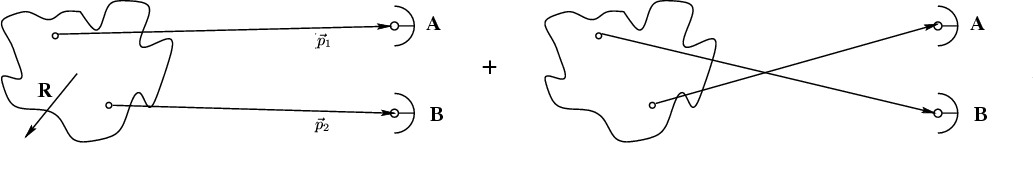
\includegraphics[width=0.9\textwidth]{wavefunction}
        \caption{The pair wave function is a superposition of all possible states. In case of particle interferometry it includes two cases: particles with momenta $p_1$,~$p_2$ registered by detectors \textit{A}, \textit{B} and $p_1$,~$p_2$ registered by \textit{B}, \textit{A} respectively.}
        \label{fig:wavefunction}
      \end{figure}
      If the particles are identical, they are also indistinguishable, therefore one has also take into account the scenario, where the particle with momentum $\vect{p_1}$ is emitted from $\vect{x_2}$ and particle $\vect{p_2}$ from $\vect{x_1}$ (Fig.~\ref{fig:wavefunction}).
      In such case, the wave function describing behaviour of a pair has to contain both components~\cite{drkisiel}:
      \begin{equation}
      \label{eq:wavefunction}
        \Psi_{ab}(\vect{q})=\frac{1}{\sqrt{2}} \left[ \exp(- i \vect{p_1}\vect{x_1} - i \vect{p_2}\vect{x_2}) \pm \exp(- i \vect{p_2}\vect{x_1} - i \vect{p_1}\vect{x_2}) \right]~.
      \end{equation}
      A two particle wave function of identical bosons is symmetric (``+'' sign in Eq.~\ref{eq:wavefunction}) and in case of identical fermions - antisymmetric (``-'' sign).
      This anti-symmetrization or symmetrization implies the correlation effect coming from the Fermi-Dirac or Bose-Einstein statistics accordingly.

      To provide full description of a system consisting of two charged hadrons, one has to include in the wave function besides quantum statistics also Coulomb and strong Final State Interactions.
      Considering identical particles systems, the quantum statistics is a main source of a correlation.
      Hence, in case of space-time analysis of particle emitting source, effects coming from the Coulomb and Strong interactions can be neglected.
    %
    % ========
    \subsection{Source emission function}
    % ========
      To describe particle emitting source, one uses a single emission function:
      \begin{equation}
        \label{eq:source-single-3d}
        S_A(\vect{x}_1,\vect{p}_1) = \int S(\vect{x}_1,\vect{p}_1,\vect{x}_2,\vect{p}_2,...,\vect{x}_N,\vect{p}_N)
        d \vect{x}_2 d \vect{p}_2 ... d \vect{x}_N d \vect{p}_N
      \end{equation}
      and a two-particle one:
      \begin{equation}
        \label{eq:source-two-3d}
        S_{AB}(\vect{x}_1,\vect{p}_1,\vect{x}_2,\vect{p}_2) = \int S(\vect{x}_1,\vect{p}_1,\vect{x}_2,\vect{p}_2,...,\vect{x}_N,\vect{p}_N)
        d \vect{x}_3 d \vect{p}_3 ... d \vect{x}_N d \vect{p}_N~.
      \end{equation}
      Emission functions $S(\cdot)$ can be interpreted as a probability to emit a particle, or a pair of particles from a given space-time point with a given momentum.

    %
    % ========
    \subsection{Theoretical correlation function}
    % ========

    %
    % ========
    \subsection{Spherical harmonics decomposition of a correlation function}
    % ========
  %
  % ========
  \section{Experimental approach}
  % ========

  % include drkisiel p. 35?

  %
  % ========
  \section{Scaling of femtoscopic radii}
  % ========

\newpage
% !TEX root = ../main.tex
% fix page break in toc
% \addtocontents{toc}{\protect\newpage}
\chapter{Results}
  %
  % ========
  \section{Identical particles correlations}
  % ========
    %
    % ========
    \subsection{Spherical harmonics components}
    % ========
      \begin{figure}[h]
        \centering
        \centerline{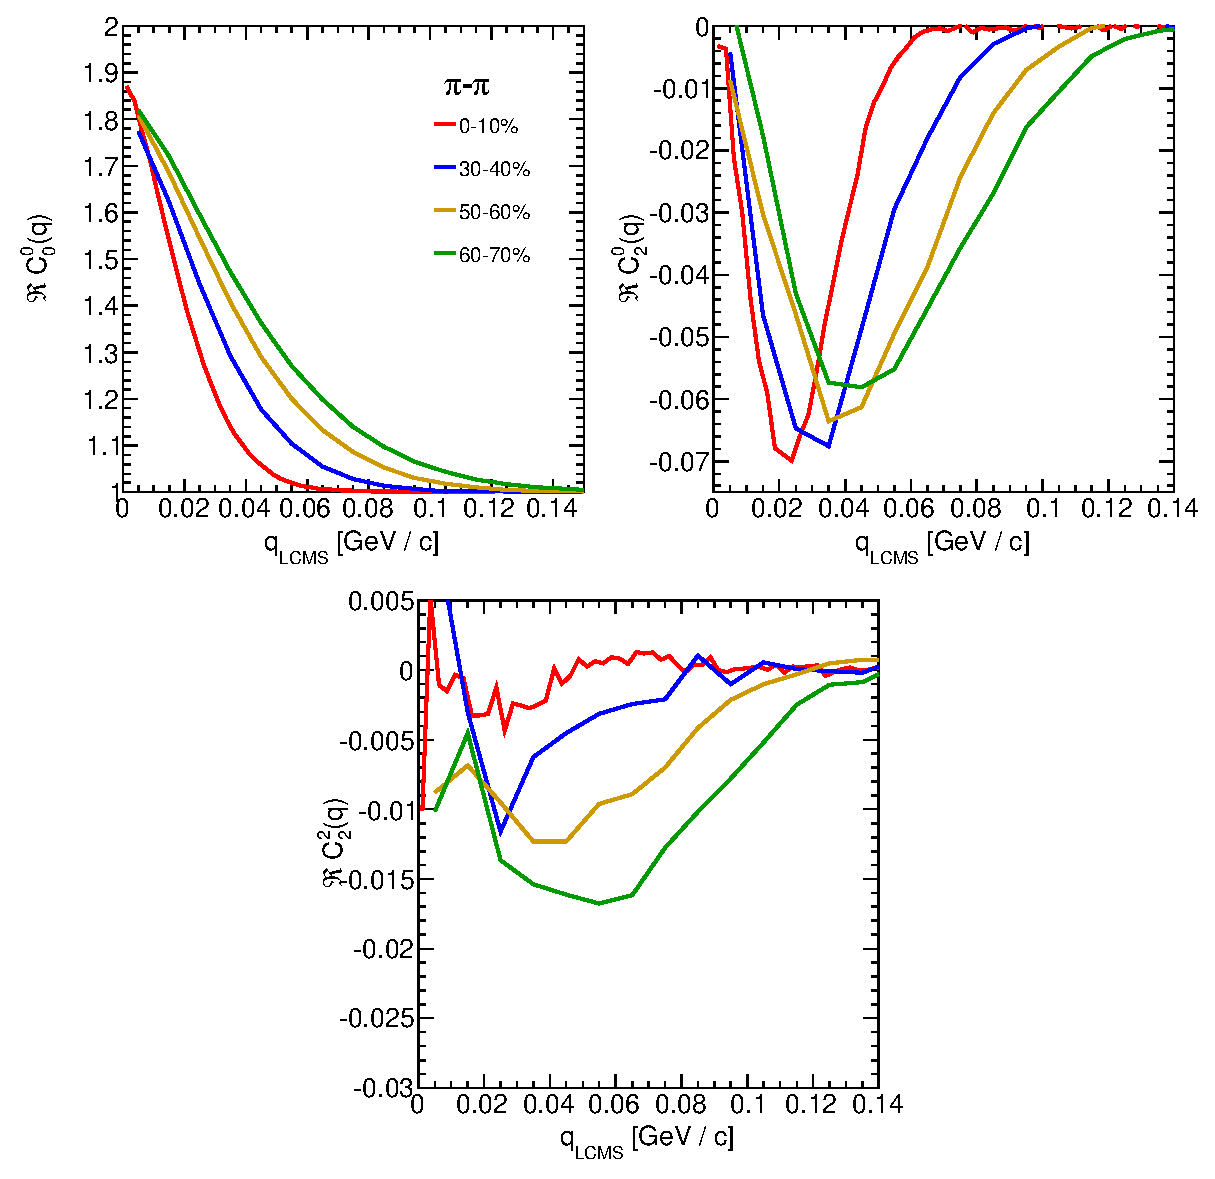
\includegraphics[width=1.1\textwidth]{results/cf3dpi}}
        \caption{no caption}
      \label{fig:cf3dpi}
      \end{figure}

      \begin{figure}[h]
        \centering
        \centerline{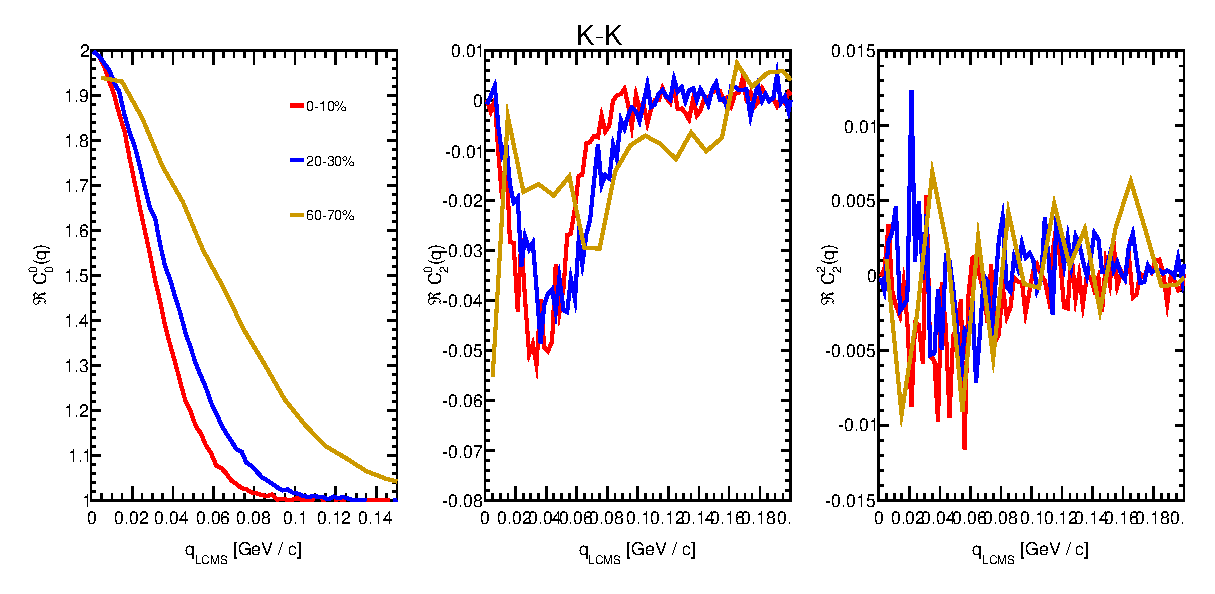
\includegraphics[width=1.1\textwidth]{results/cf3dk}}
        \caption{no caption}
      \label{fig:cf3dk}
      \end{figure} 

      \begin{figure}[h]
        \centering
        \centerline{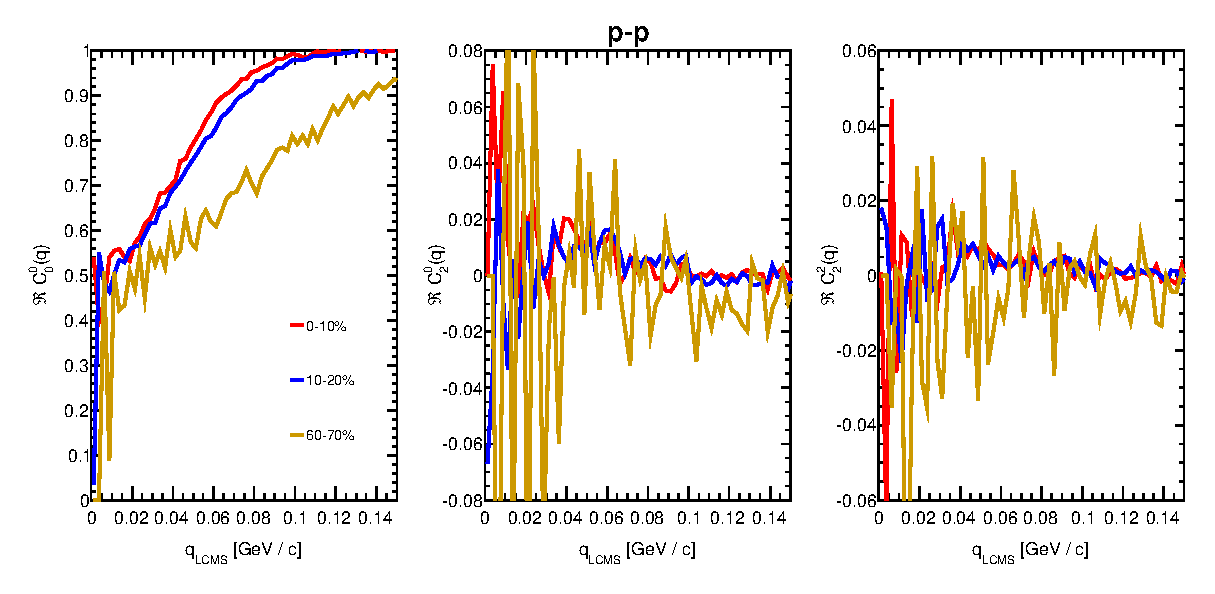
\includegraphics[width=1.1\textwidth]{results/cf3dp}}
        \caption{no caption}
      \label{fig:cf3dp}
      \end{figure}  
    \FloatBarrier
    %
    % ========
    \subsection{Centrality dependence of a correlation function}
    % ========
    % napisac o singletowym bozonow i trypletowym protonow
    % pokazac poszerzenie CF vs k_T oraz vs centralnosc
      \begin{figure}[h]
        \centering
        \centerline{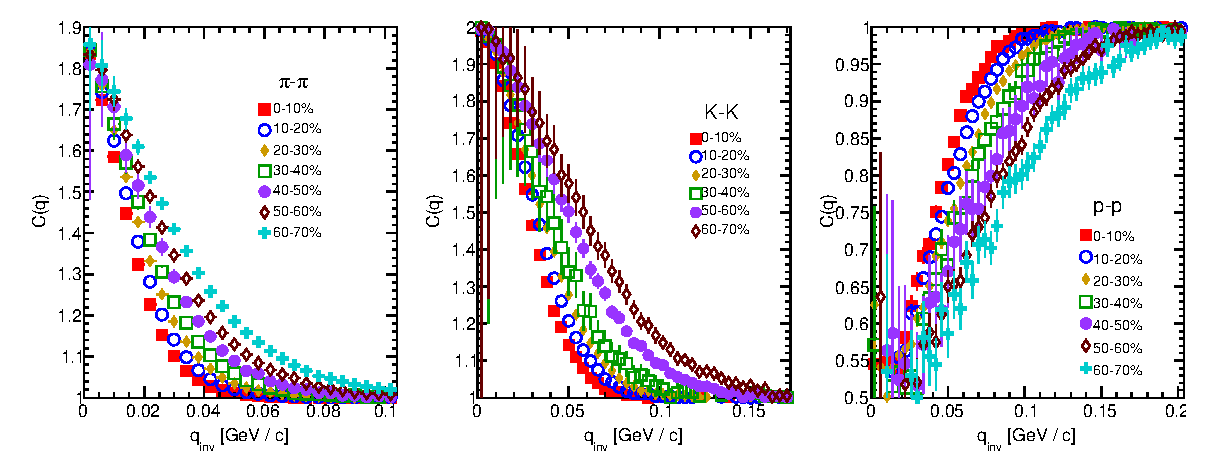
\includegraphics[width=1.1\textwidth]{results/cfvsctr}}
        \caption{no caption}
      \label{fig:centr_dep}
      \end{figure}
    \FloatBarrier
    %
    % ========
    \subsection{$k_T$ dependence of a correlation function}
    % ========
      \begin{figure}[h]
        \centering
        \centerline{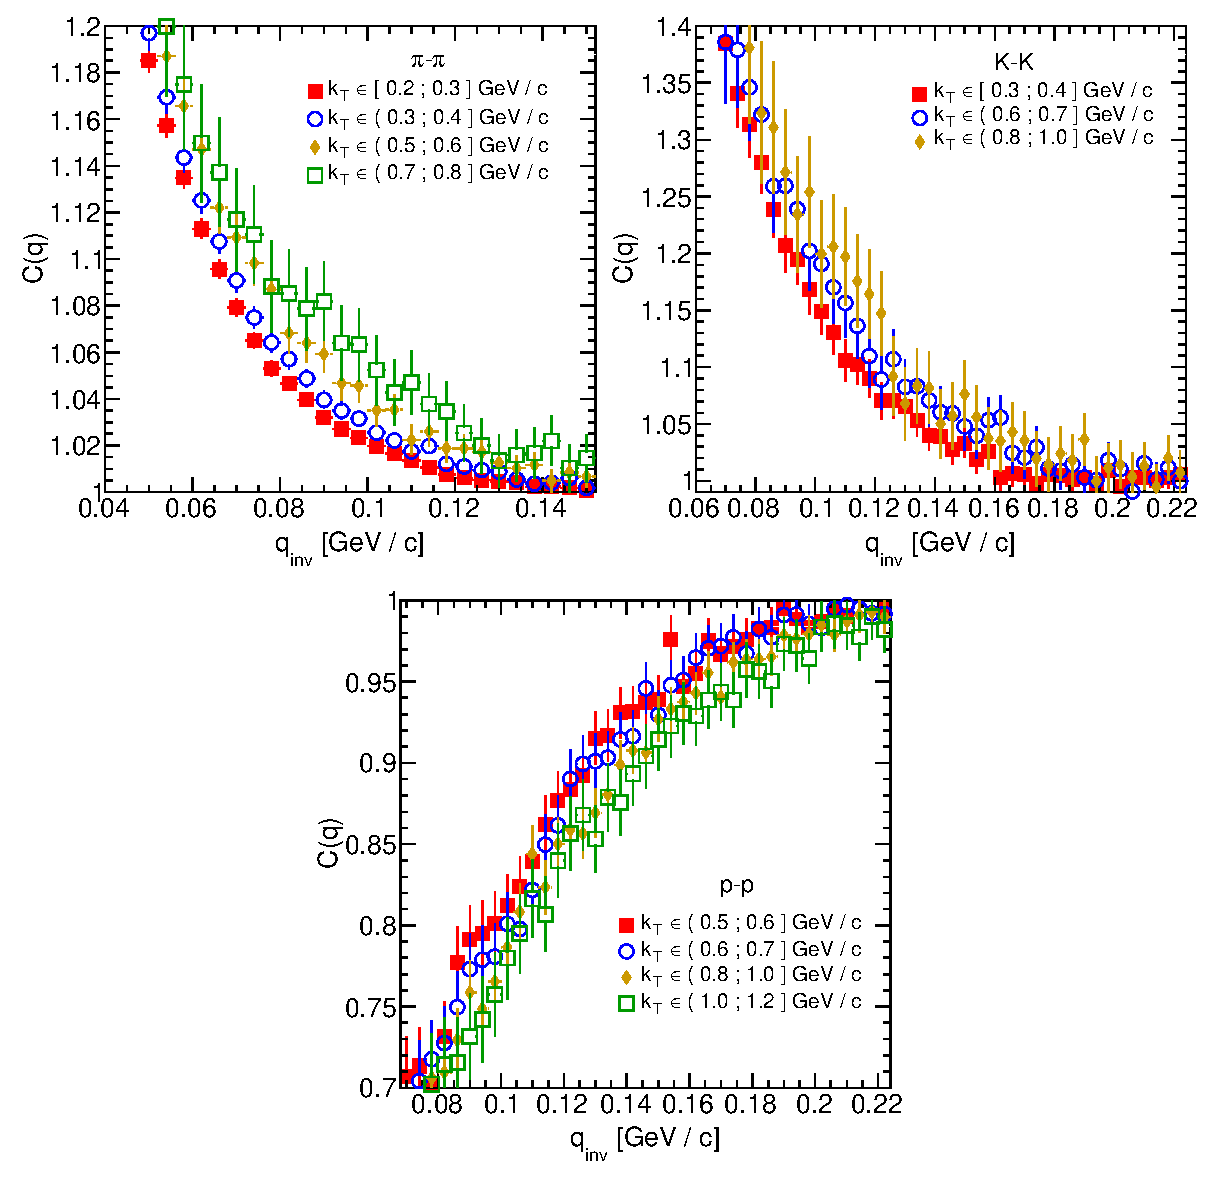
\includegraphics[width=1.1\textwidth]{results/cfvskt}}
        \caption{no caption}
      \label{fig:kt_dep}
      \end{figure}
    \FloatBarrier
  %
  % ========
  \section{Results of the fitting procedure}
  % ========
    %
    % ========
    \subsection{[] transverse mass scaling}
    % ========
    \FloatBarrier
  %
  % ========
  \section{Discussion of results}
  % ========

\newpage
\chapter{Summary}

%summary
\newpage

\bibliography{bibliography}
\bibliographystyle{unsrt}
%\listoftables
\listoffigures
%TODO rewrite statement below
%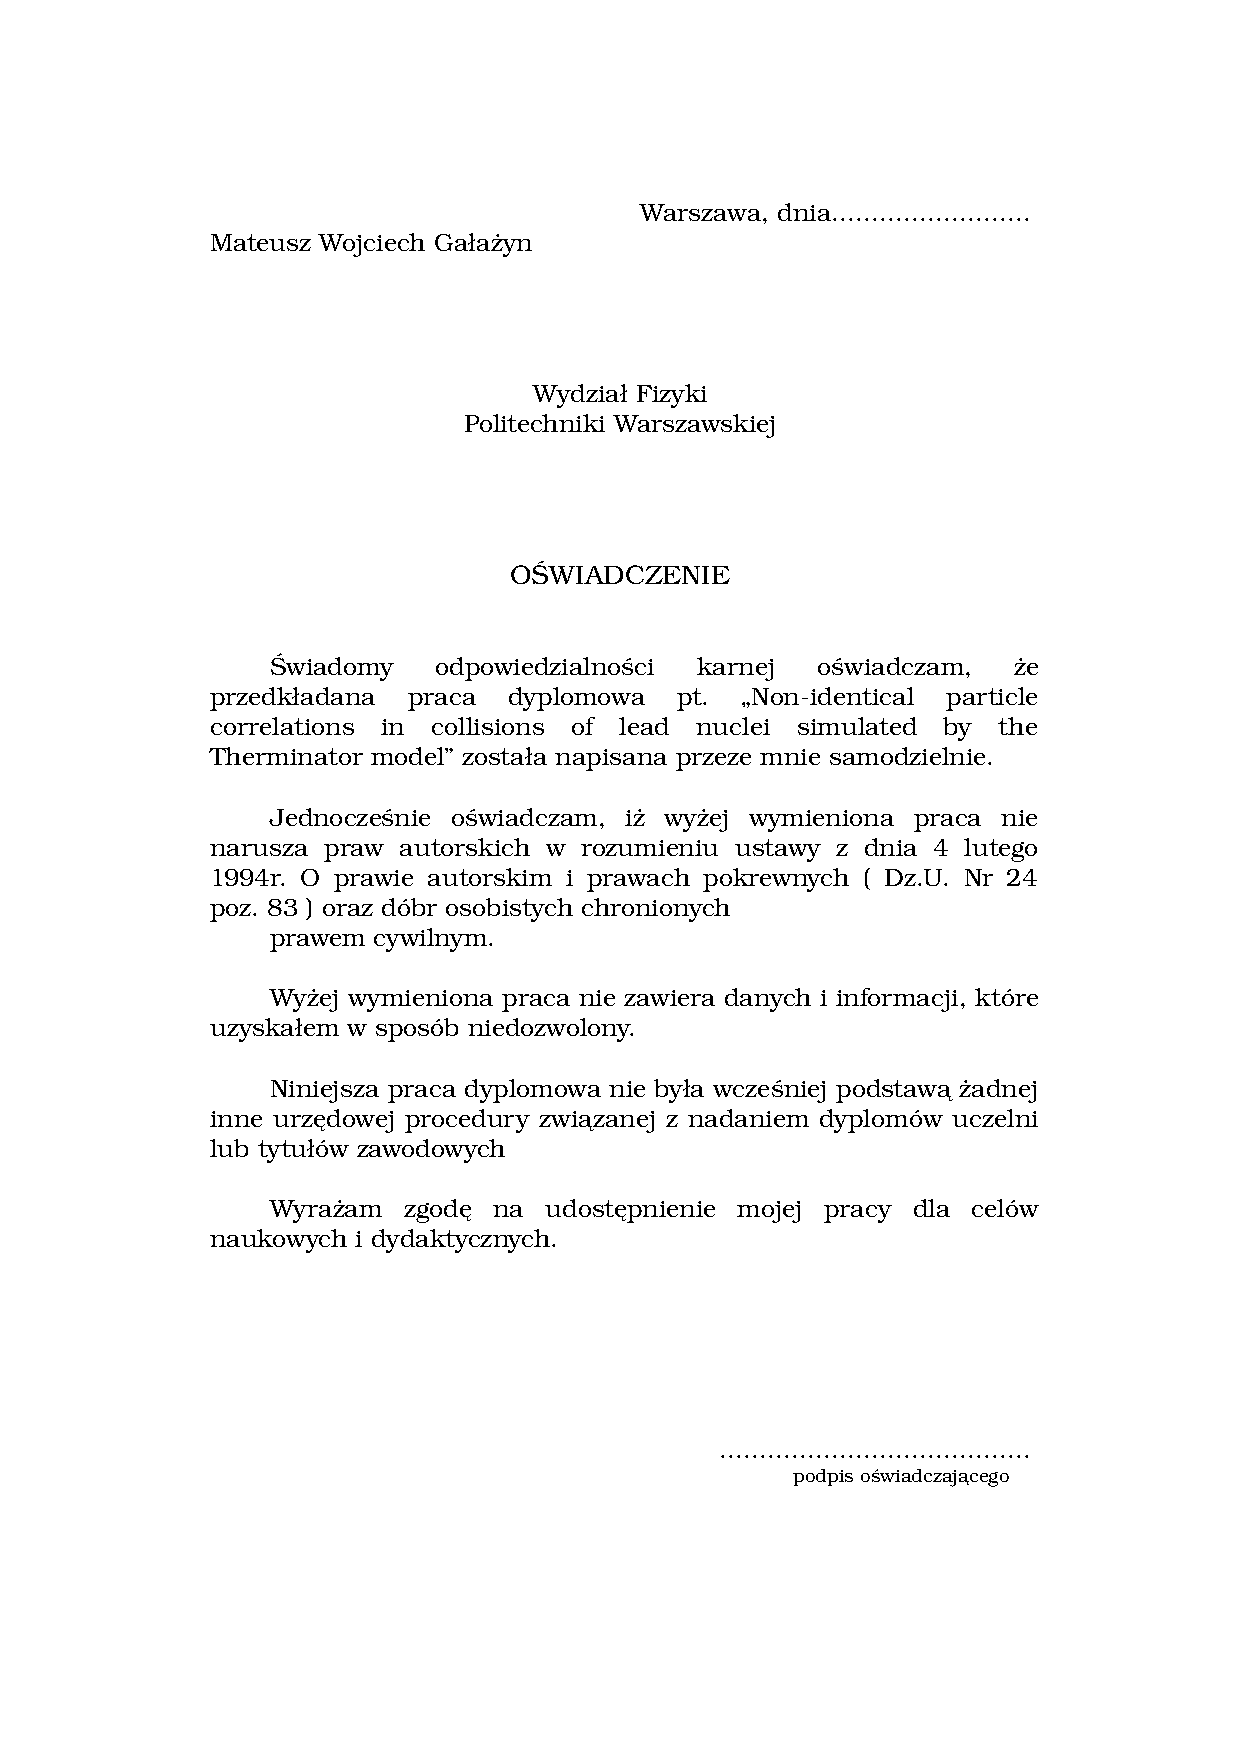
\includepdf[pages={1}]{oswiadczenie.pdf}
\end{document}